\documentclass[12pt, a4paper, openany]{book}
\usepackage[utf8]{inputenc}
\usepackage{fullpage}
\usepackage{amsmath}
\usepackage{amssymb}
\usepackage{graphicx}
\usepackage{mathtools}
\usepackage[comma,authoryear]{natbib}
\usepackage{listings}
\usepackage{color}
\usepackage{wrapfig}
\usepackage{float}
\usepackage{subcaption}
\usepackage{etoolbox}
\makeatletter
\patchcmd{\chapter}{\if@openright\cleardoublepage\else\clearpage\fi}{}{}{}
\makeatother

\definecolor{dkgreen}{rgb}{0,0.6,0}
\definecolor{gray}{rgb}{0.5,0.5,0.5}
\definecolor{mauve}{rgb}{0.58,0,0.82}

\lstset{frame=tb,
  language=R,
  aboveskip=3mm,
  belowskip=3mm,
  showstringspaces=false,
  columns=flexible,
  basicstyle={\small\ttfamily},
  numbers=none,
  numberstyle=\tiny\color{gray},
  keywordstyle=\color{blue},
  commentstyle=\color{dkgreen},
  stringstyle=\color{mauve},
  breaklines=true,
  breakatwhitespace=true,
  tabsize=3
}
\frenchspacing
\linespread{1.2}
\graphicspath{{./}}
\title{Modeling and Forecasting US Airline Flight Delays\\2020 TAMIDS Data Science Competition}
\author{Big Data Energy\\Johnathan Lo \& Isaac Ke\\Advisor: Dr. Huiyan Sang}
\date{April 8, 2020}

\newcommand{\R}{\mathbb{R}}
\newcommand{\Z}{\mathbb{Z}}
\newcommand{\Lagr}{\mathcal{L}}
\newcommand\tab[1][1cm]{\hspace*{#1}}
\pagenumbering{gobble}
\begin{document}

\maketitle
\tableofcontents

\chapter{Introduction}
\pagenumbering{arabic}
\setcounter{page}{1}
%  |||||||||||||||||||||||||||||||||||||||||||||||||||||||||||||||||||||      CHAPTER 1 [Introduction]
\tab Reliable transportation supports a strong economy by facilitating the rapid and timely exchange of goods and services and bolstering tourism revenue. In 2018, the United States transportation industry accounted for \$648 billion, which was 3.16\% of the GDP [\cite{1}]. Worldwide, the aviation industry contributes \$2.7 trillion (3.6\%) of the world's GDP. In fact, it is projected that by 2036, global air transportation will support \$5.7 trillion of the global economy [\cite{2}]. A key metric for evaluating the efficiency of airline industry production is flight delay time. In 2018, flight delays led to an economic loss of 31.2 billion dollars [\cite{3}]. For individual companies, delays can influence consumer choice, and for the industry itself, unmitigated delays can impel consumers to switch to substitute services, such as automotive or rail-based transport. \\
\tab Therefore, a major goal of this project was to analyze flight delays and diagnose areas for improvement. We intended to create models using the provided datasets as well as other publicly available data that can accurately predict future delays. In doing so, our hope was to uncover significant and controllable factors that can help guide airline companies to reduce flight delays. 
%  ||||||||||||||||||||||||||||||||||||||||||||||||||||||||||||||||       CHAPTER 2 [Executive Summary]
\chapter{Executive Summary}
%%
	\section{Problem and Approach}
\tab Ever since the first commercial airline flight was flown in 1914, the air transportation industry has played an integral part in both boosting the global economy as well as connecting people from all over the world. On occasion, flights can be delayed from their scheduled departure or arrival times, and this results in lost revenue and irritated customers. The goal of our analysis was to not only model flight delays but also create predictive models to forecast future late arrivals, specifically for the third quarter of 2019. We dove into this project by first gathering and tidying up our data, performing exploratory data analysis, then fitting and assessing unique predictive models. By gathering substantive knowledge about airlines, we then interpreted and applied our results to creating a model.  Interpretability and thoroughness were the driving forces in our analysis.
%%
	\section{Data Preprocessing}
\tab In addition to the datasets provided to us, we worked to gather historical weather information for all 11 million flights at both the origin and destination airport by fetching pertinent data from the NCDC (National Climate Data Center) API. After all data was gathered, we ensured our data was “tidy” by combining all flight, weather, airfare, route, airport, and geographical information into one data frame with each observation as a row and covariate as a column. Moreover, we changed appropriate independent variables to categorical variables, replaced all missing values with reasonable entries, and experimented with transformations of variables. For subsequent models, data were further reorganized to fit the nature of the problem. For example, for one of our models we formatted the data to resemble longitudinal panel data. 
%%
	\section{Exploratory Analysis}
\tab During the exploratory phase, we produced various plots and summary statistics to learn about the distribution and nature of flight delays. By using numerous packages in R along with connection to the Google maps API, we were able to produce numerous revealing plots. Among these, we were able to assess the geographic, temporal, carrier, and weather-based patterns of flight delays, to name a few. Through the construction of conditional density estimates and other tests, the main takeaway from our exploration was that flight delays are not a purely random event and that they behave very predictably across a myriad of factors. This motivated us to pursue the models that we did. 
%%
	\section{Model Creation \& Assessment}
\tab Using the empirical distributions found during our exploratory analysis, we created a parametric distribution for the marginal values of the response. A parametric distribution was useful here because it provided interpretability and allowed regression and Bayesian methods to be used on the parameters. A key difficulty here was the skewness of the distribution, which we could not correct through transformation methods such as Box-Cox. Attempts to fit other well-known distributions were underwhelming. Ultimately, we created out own mixture distribution, $Y = UV+(1-U)T$ where $U\sim Ber(p)$, $V\sim exp(\lambda)$, and $T\sim N(\mu, \sigma^2)$. Our parametric distribution has great descriptive utility in interpreting results. By using QQ plots and conditional density estimation, we were able to validate this parametric distribution for the majority of factor levels. Importantly, we discovered conditional densities have the same approximate distribution across factors. This distribution is henceforth referred to as the Lo-Ke distribution, named after the team members. \\
\tab Having the form of the conditional distributions allowed us to construct linear models using OLS (ordinary least squares). Observed non-normality of the errors prohibited conventional inference procedures; however, the assumptions for Gauss-Markov were not violated. To allow for prediction, we described the errors with the Lo-Ke distribution. Since the distribution is not location-scale parameterized, we instead approximated predictions by keeping other parameters constant while varying $p$. \\
\tab Next, as we found that modeling the binary variable of whether or not a delay would occur was beneficial, we trained a logistic regression model. By splitting our data into training and testing sets, we regressed on the now-binary arrival delay response on a variety of other pre-departure factors such as weather conditions. Along with critically assessing model output, we generated a Receiver Operating Characteristics curve as well as a confusion matrix to further optimize our model and maximize its accuracy. \\
\tab Lastly, we re-visited our linear model. We hypothesized that the observed pattern in the residuals might be the result of autocorrelation, or some type of time-dependency. To deal with these effects, we fitted a dynamic linear model by creating a bootstrap time series and fitting a multi-season ARIMA model (auto-regressive integrated moving average). We then fit a linear model using OLS to the residuals.
%%
	\section{Applications and Conclusions}

\tab The models we chose showed significant effects on arrival time for several different predictors. The most significant and predictable of these were seasonal effects by quarter and time of day. Flights during the 2nd and 3rd quarters were both significantly and substantially later than flights during the 1st and 4th. Time of day showed a clear effect with lower delays in the early morning, and delays peaking for flights departing around 5 PM. Day-of-week effects were also observed, with Thursday and Friday having the greatest delays. However, these differences (though significant) were not substantial. Different carriers also showed significant differences in mean arrival time. While most large airlines performed around the middle of the pack, several (notably Delta and Alaska Airlines), performed much better than expected, given their routes and revenue. Among quantitative variables, latitude, longitude, and precipitation showed usefulness as predictors. All in all, predicting flight delays involves a seasonal component as well as understanding the underlying distribution to then make predictions using the various models we developed.\\
\tab Overall, model constructing was challenging with this dataset- not only because of its size, but also because of the inherent difficulty in capturing all the possible sources of variation in flight delays. Every flight is made possible by the coalescence of hundreds, if not thousands of disparate factors; conversely, delays can result from a single anomaly among those. Most of the factors that we uncovered are out of the control of airlines themselves. 
%     ||||||||||||||||||||||||||||||||||||||||||||||||          CHAPTER 3 [Motivation, Data Description, and Sofware]
\chapter{Motivation, Data Collection, and Software \& Code}

%%
	\section{Motivation}
	\tab As stated in the introduction, flight delays can have a wide-ranging effect on the economy. Most airline companies have already done everything in their power to mitigate and reduce delays. We are interested in finding whether delays can be further alleviated, and whether those variables can be controlled by airline companies. To the extent that some delays are unavoidable or difficult to predict, we are also interested in devising methods to minimize the impact of those delays, whether by reducing the number of passengers affected, offering alternate routes to affected passengers, or discounting tickets. Overall, for the benefit of airline companies, consumers, and society-at-large, we should minimize flight delays or the impact thereof. \\
	\section{Data Collection}
%%
	\tab Our data was provided as .csv files by the competition organizers. The primary dataset was composed of roughly 11 million observations of 50 variables. Each observation was a distinct flight that occurred between 1/1/2018 and 6/30/2019. The 50 covariates included origin, destination, quarter, arrival delay, departure delay, distance, and many more variables pertaining to each flight. Auxiliary datasets included information on flight routes, airports, and market share. \\
	\tab In addition to these data, we also sought out additional information to enhance our analysis. We obtained geographic coordinates for each airport from \textit{openflights.org} and historical weather data from the NOAA databases through the NCDC API. The geographic coordinates were given in decimal format, and our weather data described meteorological events near the origin and destination of each flight. Also, a key was obtained to connect to the Google Maps API through their Google Cloud Platform. Various plots were created using this connection. A more in-depth discussion can be found in the next chapter, under \textit{Data Wrangling}.A full list of covariates along with a brief descriptions can be found in \underline{Fig 9.1} of the appendix. See \underline{Fig 9.2} for additional information on the stages and segments of air travel. \textit{From here on out, figures starting with the number 9 can be found in the attached appendix while figures starting with any other number indicate it can be found in-line with the chapter}. 
%%
	\section{Software \& Code}
	\tab All analyses were performed in R v3.6.3 using the RStudio IDE. Packages used include, but are not limited to, \textit{ggplot2}, \textit{ggmap}, \textit{dplyr}, \textit{caret}, \textit{rnoaa}, and \textit{tseries}. Individual datasets were loaded as \textit{data.frame} objects and combined using \textit{merge} along with various \textit{dplyr} commands. In addition, Microsoft Power BI was utilized in order to tidy the data and perform computationally-intensive data rearranging. The final dataset and code for this project can be found on our github repository \underline{github link}.

%      |||||||||||||||||||||||||||||||||||||||||||||||||||||||||||||||||                    CHAPTER 4 [EDA]
\chapter{Exploratory Data Analysis}
%%
	\section{Data Wrangling}
	\tab Our dataset was drawn from four different main sources - flight delays and airfare data, geographic coordinates from \textit{openflights.org}, and weather data from NOAA. Flight delays and geographic coordinates were combined by merging on both common origin and destination names. The resulting data frame was then combined with the market data by common route, year, and quarter. Adding weather data was more challenging in that the observations related information collected by weather stations, and not the airports themselves. Thus, weather station coordinates were cross referenced with airport coordinates to find the closest active weather station to each airport. Due to this constraint, 10 airports corresponding to 99,980 observations (a negligible amount given the overall size of our data), were dropped due to the lack of NOAA weather stations nearby. Weather data was then merged with the rest of the data on common dates and airports, with separate variables for weather at the origin and destination. The final dataset containing all four sets of information is what will be referenced in this paper hereafter. Small tweaks to these data were made on a model-to-model basis, depending on the type of unique problem selected-whether it be classification or regression, for example. \\
	\tab The data contained a number of variables with numerical values that could be interpreted either as quantitative or categorical variables. Using substantive knowledge, a number of numeric variables were converted to factors, including day of week, month, quarter, and route number. Additionally, our data contained many missing values. Where applicable, missing categorical variable values were replaced by adding an additional factor level \textit{Unk}. For quantitative variables, missing values were either replaced with 0 or observations were removed entirely based on substantive knowledge of the variable characteristics. Finally, we discovered that the flight delay dataset somewhat bewilderingly assigned canceled flights a delay time of 0. Canceled flights were removed from the dataset and analyzed separately. Throughout this report, we further to flight delays as specifically arrival delays as opposed to departure delays. In all, the final dataset consisted of 10,614,150 observations of 100 variables. 
%%
	\section{Distribution of Flight Delays}
	\tab The dataset provided information on flights from 17 different carriers along 6,684 unique routes being flown between a combination of 362 airports in the United States (including Alaska and Hawaii and a couple airports in US territories such as Guam). 3,814,366 out of the 10,915,495 flights (35\%) had some form of arrival delay. A histogram of all arrival delays is shown in \underline{Fig 4.1}. We observe that most "early" flights are not incredibly early compared to the frequency at which late flights can become "significantly" delayed, say more than 30 minutes. Clearly, the data is strongly right-skewed. To correct the skewness (to meet assumptions for our analysis), a cube-root transformation was performed. Subsequent Shapiro-Wilk tests provided strong evidence against normality for this transformation, so we turned to other methods, as will be discussed in chapter 5. To heuristically assess dependence between covariates and late arrivals, we examined various conditional distributions, as follows.\\
	\begin{wrapfigure}{l}{0.55\textwidth}
	\centering
	 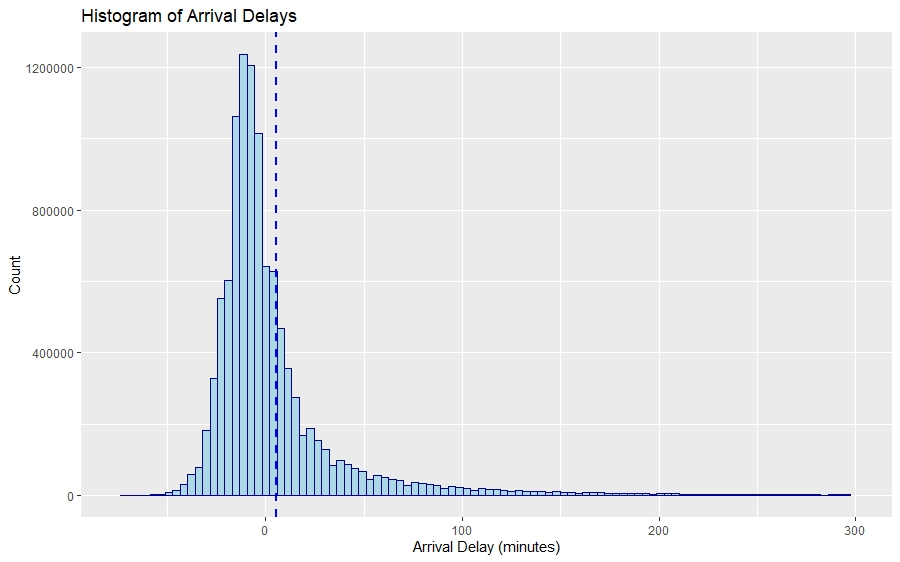
\includegraphics[width = .5 \textwidth, height = 8cm]{../figures/PLOTS FOR REPORT/Chapter 4/Figure 4.1}
	 \caption{Histogram of arrival delays for all observations in the dataset. The dashed line depicts the mean.}
	 \end{wrapfigure}
%%%	 
		\subsection{Geographic Distribution of Flight Delays}
		
			\tab In \underline{Fig 4.2}, the routes that have various average intervals of delay time are shown. Note straight lines are drawn for simplicity; the actual flight most likely flew a non-linear path toward the destination. Also, early arrivals are given a delay time of 0 in the computation of the mean. We observe many things. Almost all routes have an average delay that is positive. This spotlights the nature of this project: to focus on remedying delays to improve customer satisfaction and increase airline revenue.
			\begin{figure}[h]
			\centering
	 		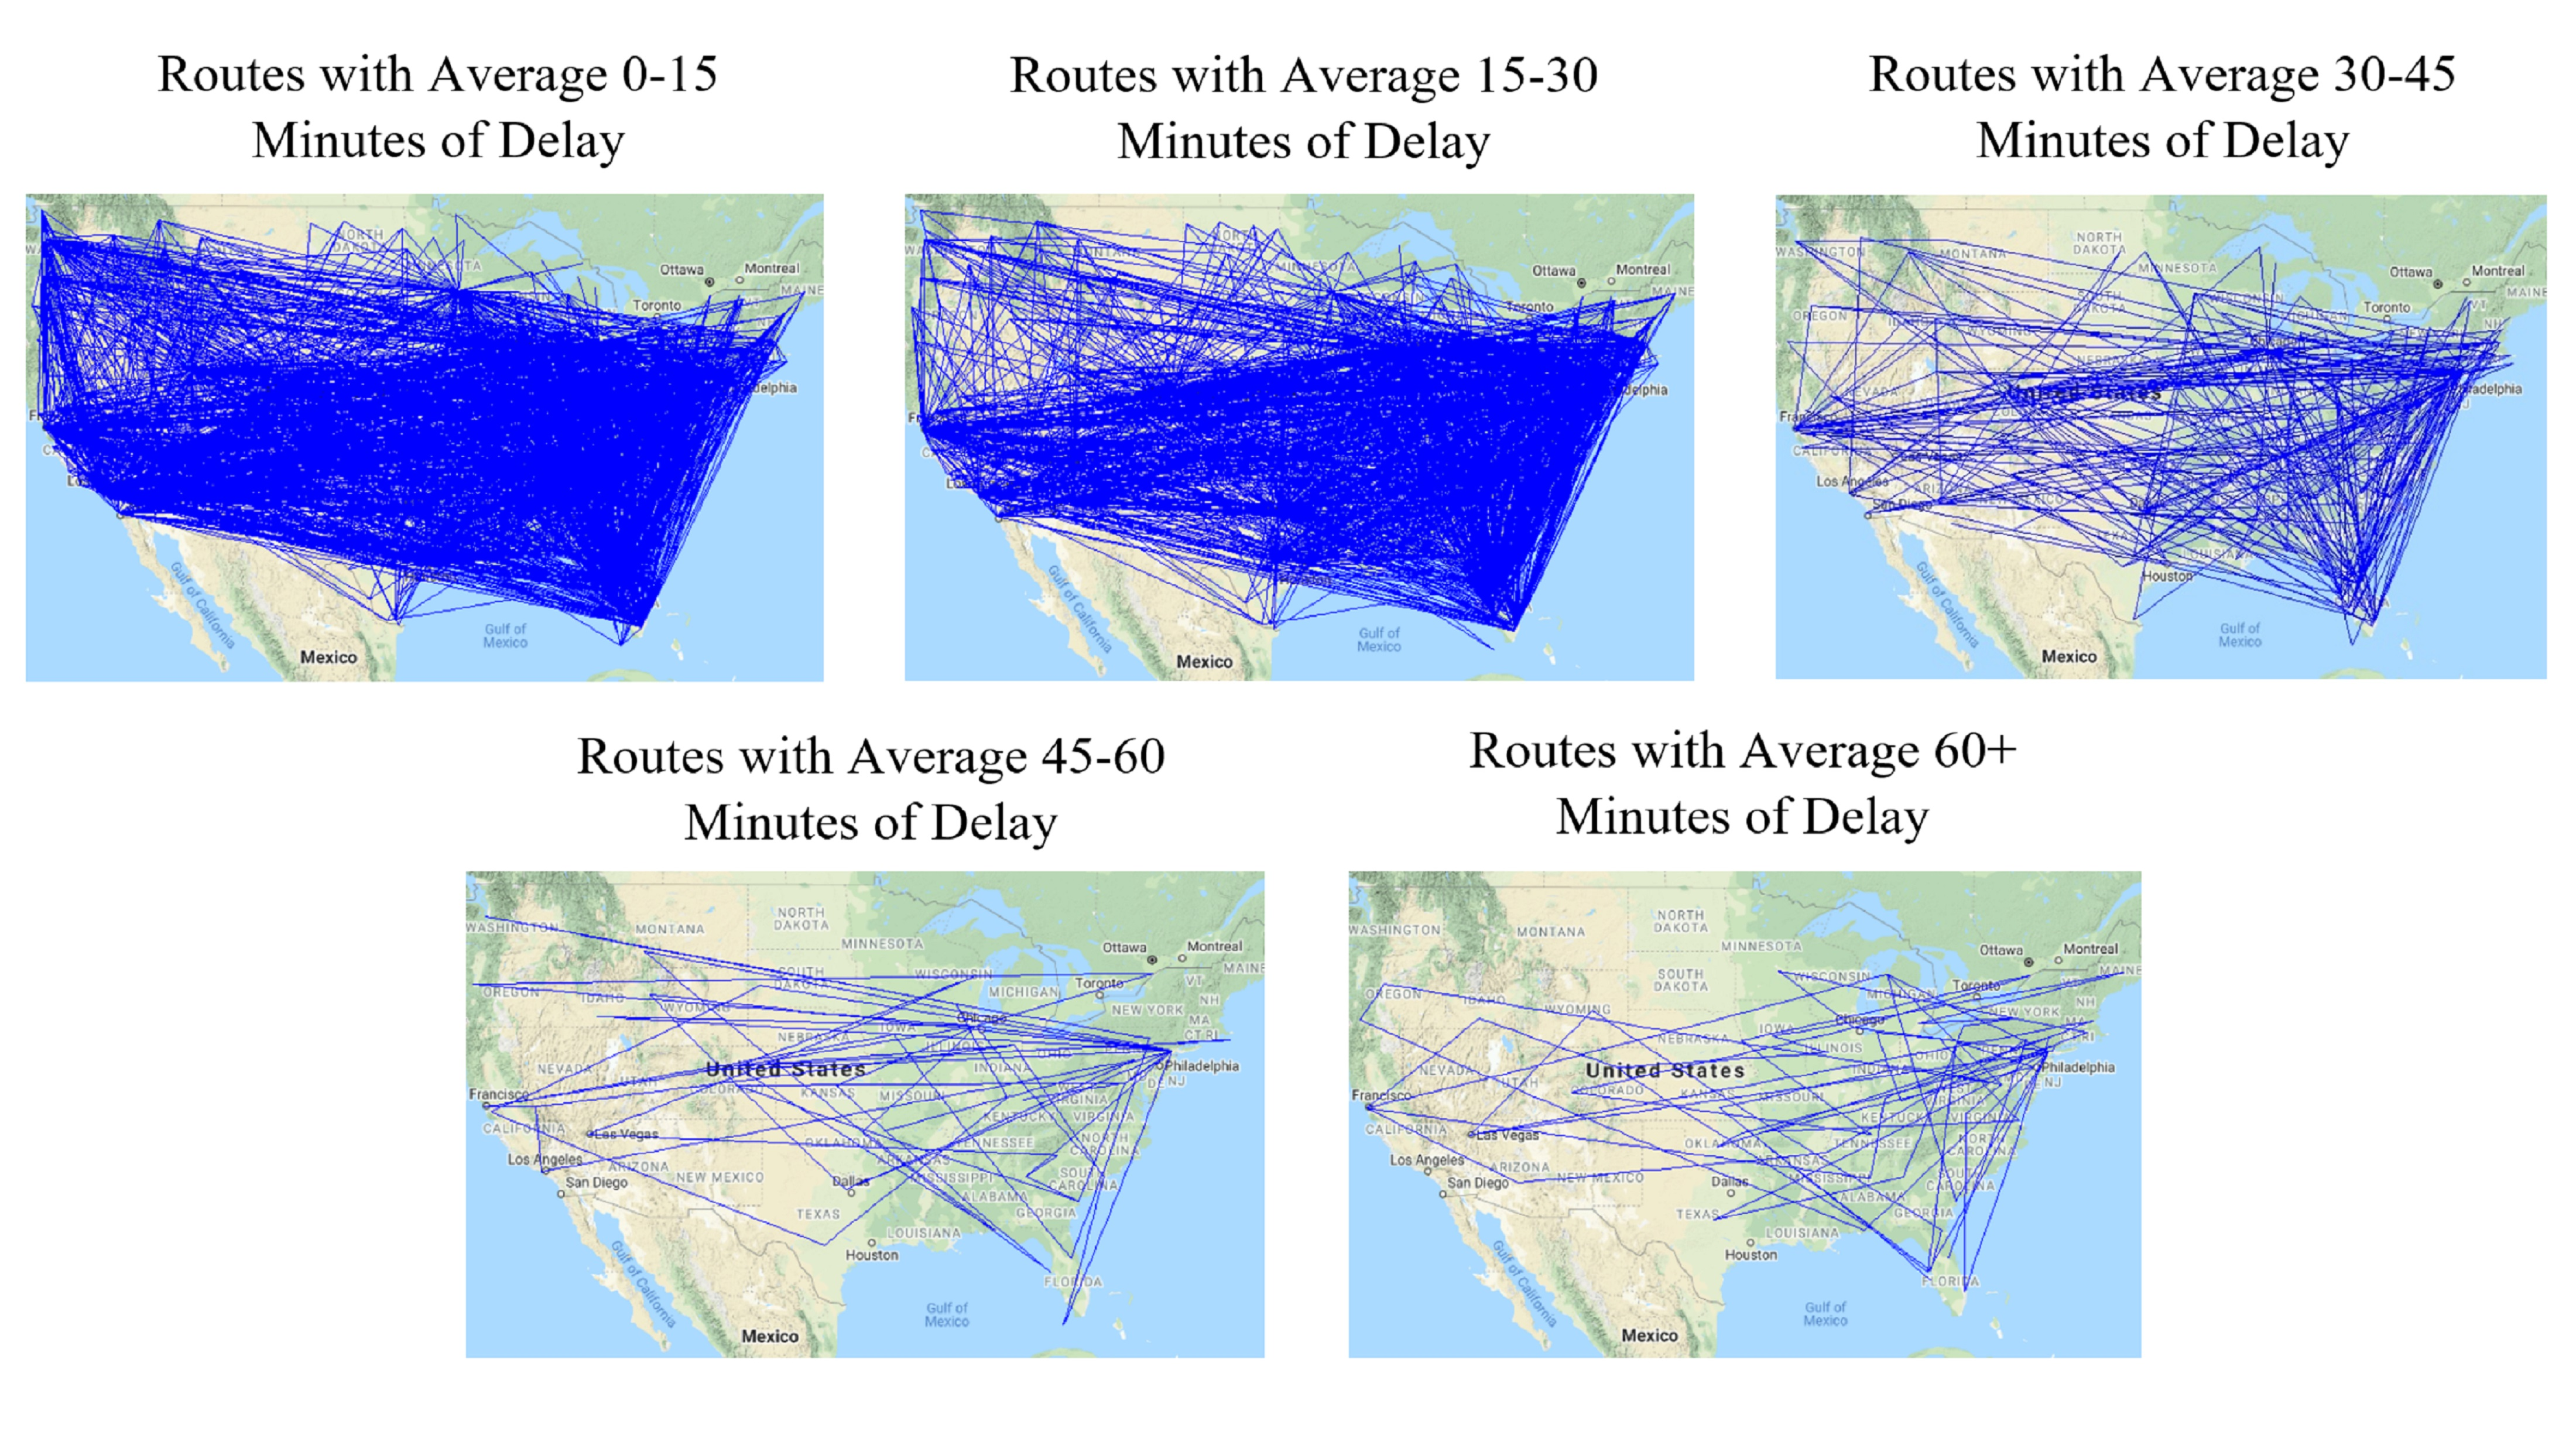
\includegraphics[width = .9 \textwidth]{../figures/PLOTS FOR REPORT/Chapter 4/Figure 4.21}
	 		\caption{Routes with different averages of delay time}
	 		\end{figure}\\

	 		\tab For the routes with a mean delay between 30 and 45 minutes, most of the delays are clustered on the eastern US with most of the routes either beginning or ending in the San Francisco, New York, or southern Florida regions. For more severe delays of 45+ minutes, these routes encompass more cross-country flights. Furthermore, it can be seen that an airport in the northeast, most likely JFK in New York, is involved in a lot of severe flight delays. In \underline{Fig 9.3}, the average delays at certain airports is depicted. We see further evidence that the more problematic delays are centered in bigger cities, particularly those on the east and west coast. \underline{Fig 9.4} illustrates the relationship between the popularity of an airport and the amount of delays. As expected, airports that crank out more flights have a higher average delay time. This raises the question: Do more flights simply give airports a higher probability of having delays (by random chance), or does an increase in flights also bring in other factors that \textit{cause} an increase in flight delays? In more broad terms, what factors correlate with delays and which ones can be controlled by the airlines?\\
%%%
		\subsection{Temporal Distribution of Flight Delays}

		\begin{figure}
		\centering
		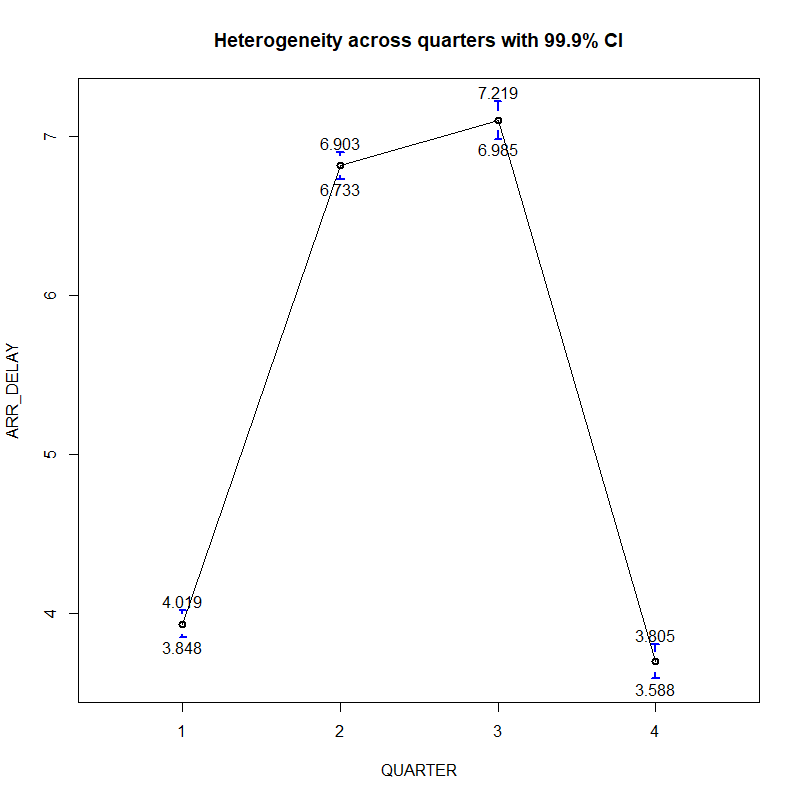
\includegraphics[width = .33 \textwidth]{../figures/heterogeneity_quarters}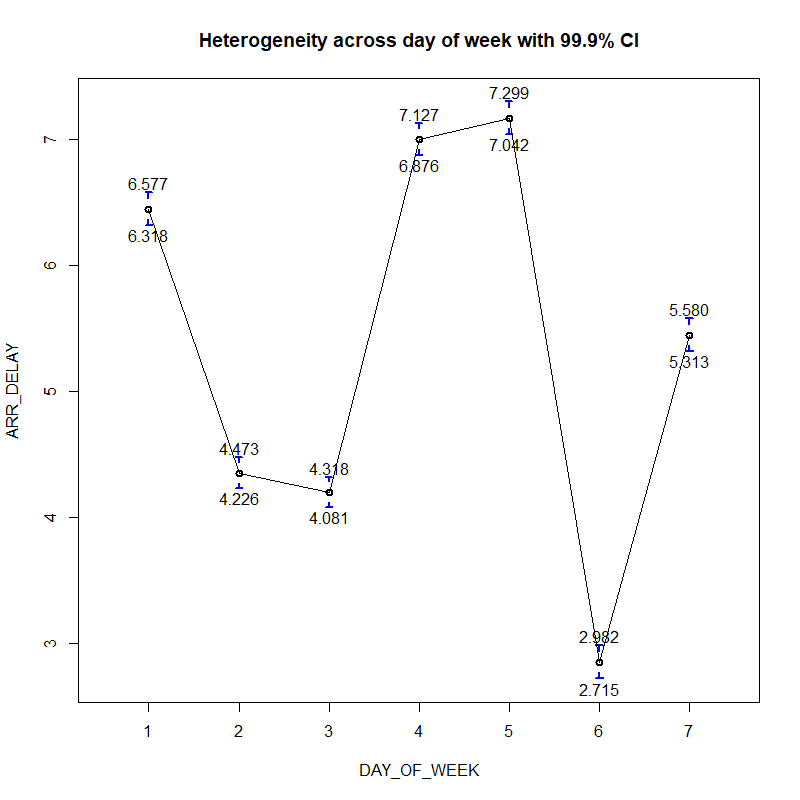
\includegraphics[width = .33 \textwidth]{../figures/heterogeneity_dayofweek}\\ 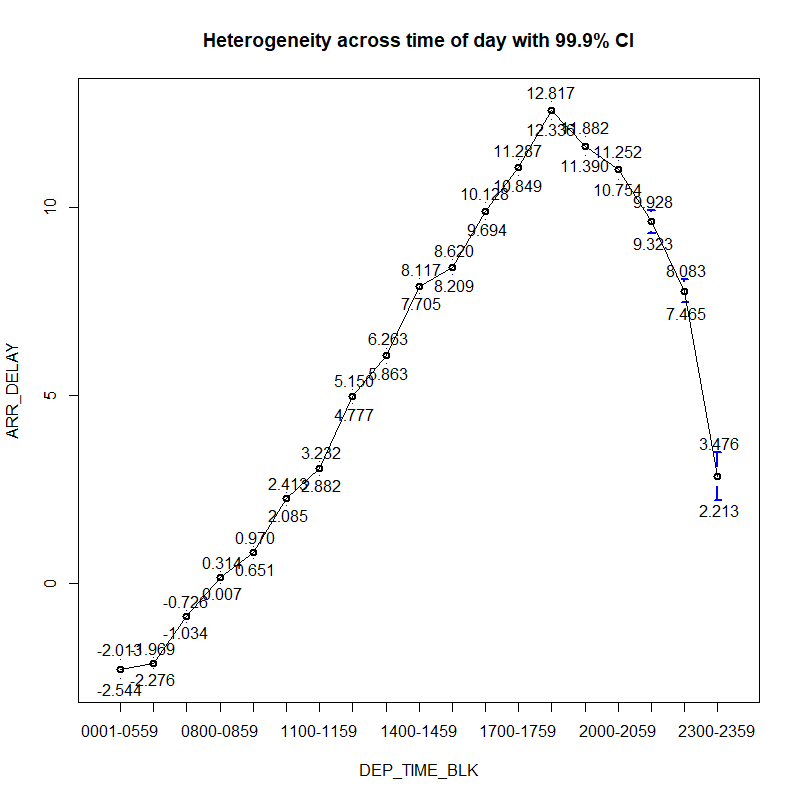
\includegraphics[width = .33 \textwidth]{../figures/heterogeneity_timeofday}
		\caption{Heterogeneity by quarter, day of week, and time of day}
		\end{figure}
			\tab \underline{Fig 9.5} shows the distribution of flight delays by quarter. Note the similarity of the marginal distributions. Distributions by month, day of week, and time of day are shown in \underline{Fig 9.6 - Fig 9.8}. Note that because our data contained a year and a half’s worth of observations, the frequency of delays for quarter 1 and 2 are higher than other time periods that were not recorded twice. The histograms appear roughly symmetric with a slight right-skew. Specifically, early arrivals appear to follow a normal distribution while it transitions to an exponential distribution once delays become positive. We will explore this specific observation in the first section of our next chapter. Regardless, the general form of the distribution across these time factors does not change significantly. \\
	
	
		
	To further investigate the role of temporal factors in flight delays, we produced a number of coplots, which show several interesting seasonal patterns, as depicted in \underline{Fig 4.3}. Namely, the most problematic times for delays are quarter 2 and 3, Thursdays and Fridays, and around 5PM-6PM in the evening.\\	 
%%%		
		\subsection{Weather-based Distribution of Flight Delays}
			\begin{figure}[h]
			\centering
	 		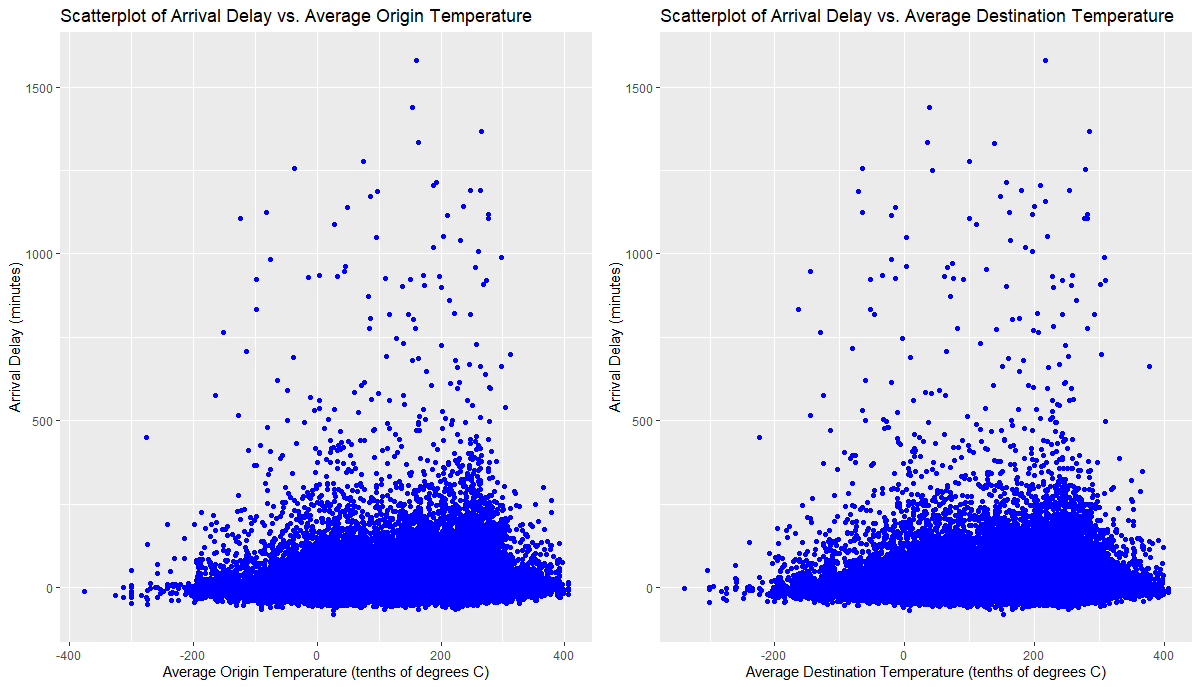
\includegraphics[width = .9 \textwidth]{../figures/PLOTS FOR REPORT/Chapter 4/Figure 4.41}
	 		\caption{Delays vs. Temperature}
	 		\end{figure}

	\tab Intuitively, the most obvious factor that most likely affects flight delays is the weather. Therefore, we analyzed the conditional distributions of flight delays given average temperature, precipitation, snow, and the presence of various rare weather events. These are described in \underline{Fig 4.4}, \underline{Fig 9.9}, and \underline{Fig 9.10}, respectively. In the scatterplot depicting rain, we see a lack of evidence that more extreme temperatures correlate with increased delays. This would be supported if the scatterplot showed a parabolic pattern, which is not seen. Surprisingly, we see the same idea in the scatterplot of precipitation. Contrary to intuition, as the amount of precipitation increases, there is no visual subsequent increase in the delay time. Lastly, \underline{Fig 9.10} demonstrates that some dangerous weather events have a slightly bigger effect on delay times than others. For example, the distributions of “ice, sleet and hail” and “blowing or drifting snow” have more area in their right-tails. This is indicative of more occurrences where these events caused more significant delays. Besides these difference in tail-density, the overall shape remains very similar. \\
%%%
		\subsection{Carrier-based Distribution of Flight Delays}
			
			\tab Next, looking at delays by carrier would provide us with insight as to whether some carriers are better at mitigating delays than others. \underline{Fig 9.11} shows us that the distribution across carriers stays roughly the same. Apart from the differences in frequencies (with some airlines being more popular or providing more flight routes), the shape of the distribution is basically homogeneous, especially when compared to the other conditional distributions of other factors. This means that delays across carriers \textit{behave} in the same manner. To analyze if the average delay time (as opposed to the distribution) differs across airlines, we conducted ANOVA (analysis of variance). Specifically, we used Tukey’s HSD to make multiple comparisons across each combination of carriers to see what carriers differed from one another. A plot of the resultant 95\% confidence intervals for the mean difference between airport delays is show in \underline{Fig 9.12}. We see that the majority of the intervals constructed do not fall within 0. Thus for those that didn’t, we conclude that they do indeed have a difference in mean arrival delays. All in all, we observe that the \textit{distribution} across carriers is similar, but the \textit{quantitative amount of delays} across carriers is different. \\

%%%
		\subsection{Airport-based Distribution of Flight Delays}
			
			\tab \underline{Fig 9.13} displays the histograms of delays for some of the most popular airports. As has been the trend thus far, the distribution across the airports does not change much save for the changes in frequency. Thus, we can conclude the behavior and process of flight delays is pretty universal and can be modeled with an explicitly defined distribution, as we will dive into in the next chapter. \\
			\tab Additional plots from conditional density estimation can be found in the appendix.  
%%%
		\subsection{Making Up Lost Time En Route}
			\tab One last thing we wanted to explore was the ability for pilots to make up lost time as a result of a departure delay. We presumed that a longer flight, distance-wise, would allow for more opportunity for a flight delay to be alleviated. In the air, harnessing favorable air currents or taking shortcuts can remedy the lost time they left the ground with. Surely, in \underline{Fig 4.5}, we see that flights over a longer distance have, on average, less arrival delays. Similarly, the shorter the flight, the more severe the arrival delay is. These observations support our hypothesis stated above. Of course, correlation does not imply causation, so more substantive knowledge on how pilots navigate the flight route would provide more clarification on this. \\
			\begin{wrapfigure}{l}{0.75\textwidth}
			\centering
	 		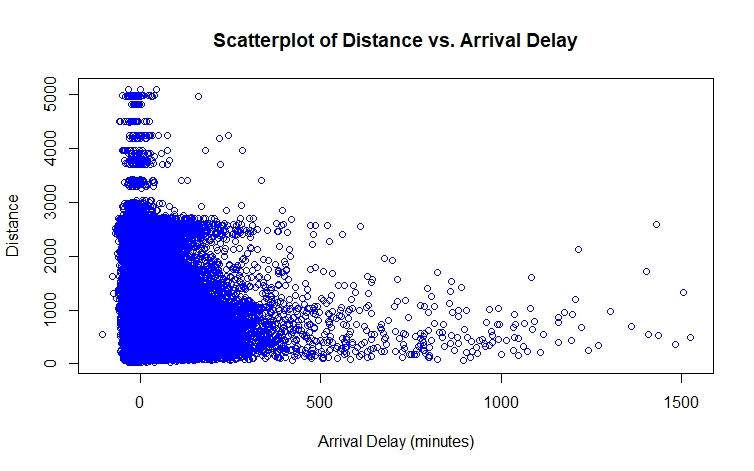
\includegraphics[width = 0.75 \textwidth]{../figures/PLOTS FOR REPORT/Chapter 4/Figure 4.8}
	 		\caption{Do longer flights allow for lost departure time to be made up?}
	 		\end{wrapfigure}
%      ||||||||||||||||||||||||||||||||||||||||||||||||||||||||        CHAPTER 5 [Model Formulation and Assessment]
\chapter{Model Formulation and Assessment}
%%
	\section{Constructing a Parametric Distribution for \\Delays}
	 \tab Fresh off our exploratory analysis, we were primarily interested in deducing the marginal distribution of arrival times from the data. Although it would have been relatively facile to estimate a valid empirical distribution, we decided that a parametric distribution would be more useful and intuitive. By establishing a set of parameters, further work could be directed towards estimating parameters under certain combinations of covariate values. With mostly categorical data, it then became feasible to estimate parameters for certain combinations of interesting variables. Parameterization also allows the density functions of the distribution to be expressed analytically.\\
	 		\begin{wrapfigure}{l}{0.35\textwidth}
			\centering
	 		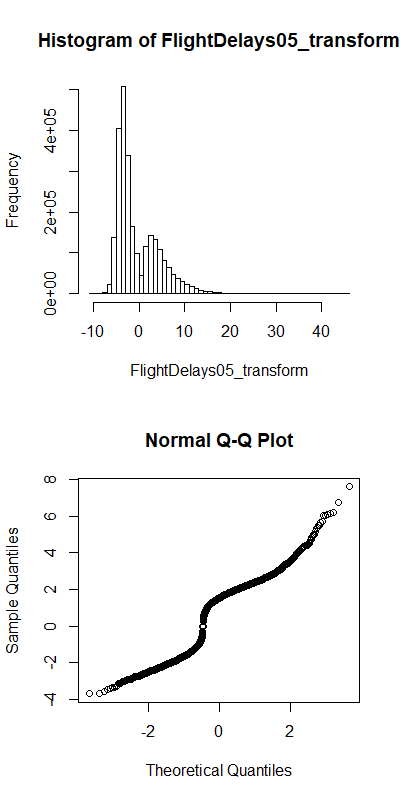
\includegraphics[width = .35 \textwidth]{../figures/shittysqrt}
	 		\caption{Density plot of square root transformation vs normal distribution with same mean and variance}
	 		\end{wrapfigure}

	\tab As seen in \underline{Fig 4.1}, the marginal distribution is strongly right skewed, and thus our first plan of action was to attempt a transformation to correct the skewness. A number of transformations were considered. With negative values in the data, log or square root transformations could only be applied by first shifting the data to be strictly positive. One way to do this was to simply add the smallest (most negative) number to each of our delay times; however, it was decided that this approach rendered our results somewhat uninterpretable. Consider, for example, a new observation where the flight arrived earlier (with a negative flight delay) than any other flight in the dataset. Such an observation would not be supported in a distribution of log-transformed values. We also briefly considered cube root transformation, but as seen in \underline{Fig 5.1}, it did not result in normality or resemblance to any familiar parametric distribution. In lieu of transforming the data, we considered several well-known skewed distributions, but none of them fit well or appeared sensible.\\

	\tab Thus, we instead looked to construct a mixture distribution. The primary issue that we had been confronted with thus far was finding a distribution that appeared to have sensible parameterizations.  Our search was rooted in the premise that not all delays are created equal. We suspected that the majority of delays are "run-of-the-mill" events that do not result from any extraordinary circumstances in particular, while a minority of delays have true substantial causes. This is similar to the rationale for a zero-inflated Poisson distribution used in manufacturing processes. This famous distribution assumes most machines are in good working order and do not produce any products with defects, but some machines with defects will produce problematic products by a Poisson distribution. \\
	\tab In this vein, we decided upon a mixture of the form \begin{center}$$Y = UV + (1-U)T$$\end{center} with $U\sim Ber(p)$, $V\sim exp(\lambda)$, and $T\sim  N(\mu,\sigma^2)$. In this model, $U$ describes whether or not a delay with "true, substantial causes" occurs, $T$ describes the distribution of arrival times when no extenuating circumstances occur, and $V$ describes arrival times under defined circumstances that result in lateness. The cumulative distribution function (CDF) of this distribution is given by 
	\begin{center}$$F_X(x) = \sum \alpha_i F_i(x) = p(1-e^{-\lambda x}) + (1-p)\left(\frac{1}{2}(1+ erf(\frac{x-\mu}{\sigma\sqrt{2}}))\right)$$\end{center}
	e.g. a simple mixture of two distributions. The complementary probability density function (PDF) is given by \begin{center}
	$$f_X(x) = F_X'(x) = p(\lambda e^{-\lambda x} ) + (1-p)\left(\frac{1}{\sigma \sqrt{2\pi}} e^{-\frac{1}{2}(\frac{x-\mu}{\sigma})^2}\right)$$
	\end{center}
	To estimate our parameters, we constructed functions in R to perform maximum likelihood estimation for our distribution.  Using \textit{optim()} in R, we were able to generate estimates of the parameters for the marginal data, as shown in \underline{Fig 5.2}.\\
	 		\begin{wrapfigure}{l}{0.35\textwidth}
			\centering
	 		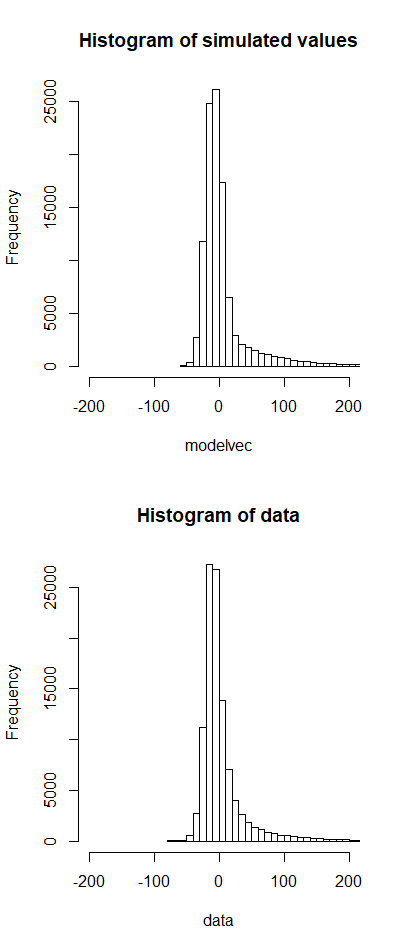
\includegraphics[width = .35 \textwidth]{../figures/MarginalMLEHist}
	 		\caption{Theoretical marginal density vs empirical marginal density}
	 		\end{wrapfigure}
	\tab We decided to name this distribution the Lo-Ke disitrbution after the members of this team who formulated it. To validate this distribution, a QQ plot was made of the observed arrival delays distribution against our Lo-Ke distribution under the parameter estimates from the MLE (\underline{Fig. 5.3}). From this plot, it can be observed that our mixture distribution is elegantly able to describe the observed values of arrival time quite accurately. The points hugging the diagonal line mean that the quantiles on our custom distribution match up with the quantiles of the data. Note that the arrival times are given as discrete values (in minutes), hence the "jumps" from percentile to percentile. It is important to note here that our distribution is not as strong in describing data points in the extreme upper range of observations, p<.001. Some delays were quite extreme, with values in excess of 1,000 minutes. To prevent such outliers from having undesired effect on our downstream analyses, we further pared the dataset here to include only data below the 99th percentile.  \\
			\begin{wrapfigure}{r}{0.45\textwidth}
			\centering
	 		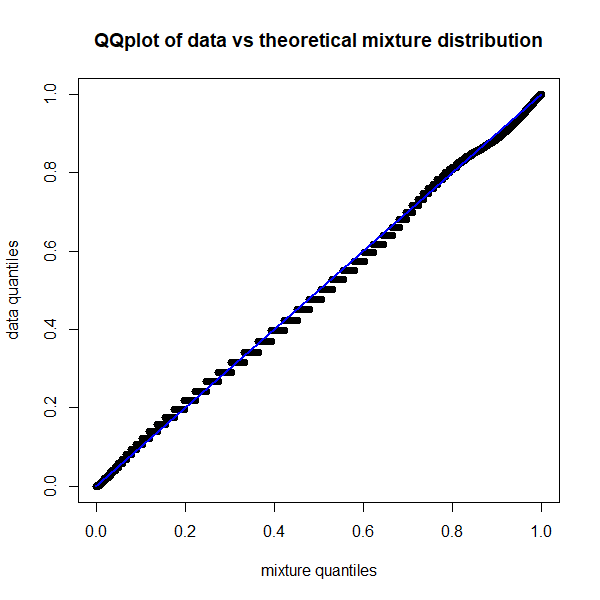
\includegraphics[width = .45 \textwidth]{../figures/QQplot-marginaldata}
	 		\caption{QQ plot of of data vs theoretical distribution}
	 		\end{wrapfigure}
	\tab Further, we see that conditional density estimation agrees with our theoretical parametric distribution. In \underline{Fig 5.4}, we show the marginal distribution for a subset of flights out of ABE, and compare it to the theoretical distribution constructed with MLE. Additional examples of the empirical conditional density vs our MLE estimates are shown in \underline{Figs 5.5, 5.6}. Overall, we suggest that our theoretical Lo-Ke distribution can be used to accurately describe arrival delays across all combinations of factor levels. \\

%%
	\section{Linear Model Using OLS}
	\tab Ideally, when constructing a linear model using OLS (ordinary least squares) estimates, we want to satisfy four principal assumptions. Namely, these are: linear relationship between predictors and responses, independence of errors, homoscedasticity, and normality of the errors. However, having seen that the conditional distributions of the response are strongly \textit{non-normal} and that there exists no simple transformation to restore normality, the fourth assumption appears to be violated. It is important to remember then, that the Gauss-Markov theorem does \textit{not} require normality of the errors for the OLS estimates to be the best linear unbiased estimator and that normally distributed errors are required only for conducting inference on the model via the t-distribution. For merely constructing a model equation and generating predictions that minimize the mean squared error, normality of the errors is not strictly required. Further, inference on the model parameters can still be conducted through a variety of alternative methods. With heavy-tailed distributions of residuals, usually the more general M-estimation is used in place of OLS estimation to provide robustness against non-normality when conducting hypothesis tests on model parameters. Alternatively, bootstrap can be used to generate the empirical error distribution. However, the size of our dataset obviates the need for either of these procedures since we can reasonably assume by the Central Limit Theorem that our estimates of the mean response, and therefore the coefficients of the model, are normally distributed. Therefore, the only inference that cannot be performed with the usual set of equations is prediction. \\
	\tab To conduct prediction and construct prediction intervals, we use our theoretical Lo-Ke distribution to describe the errors. The predictions thus have the form: \begin{center}
	$$Y_{new}|X\sim X\beta + e$$
	with variance
	$$Var(Y_{new}|X) = X^TXVar(\beta) + Var(e)$$
	and
	$$E(Y_{new}|X) = E(X\beta)$$
	\end{center} 
	\tab The question then becomes how to select parameters for the theoretical distribution of our conditional responses. Particularly, how do the parameters relate to the mean and variance given above?  For errors that are normally distributed, or distributed via some member of the location-scale family of distributions, the parameters are precisely those given by the variance and expectation above. However, for our Lo-Ke distribution, solving for the correct parameter values becomes more challenging. Analytically, this requires either solving for the method of moments estimators or the maximum likelihood estimators. Both analytical solutions become complex rather quickly. For example, we calculated the following moments of our theoretical distribution:
	\begin{center}
	$$M_1 = \frac{p}{\lambda} +(1- p)\mu$$
	$$M_2 = p\left(\frac{2}{\lambda^2} - \frac{2\mu+1}{\lambda} - \mu^2 - \sigma^2\right) +\mu^2 +\sigma^2$$
	$$M_3 = \frac{6p}{\lambda^3} -(p+1)(\mu^3 + 3\mu\sigma^2) $$
	\end{center} 
	where we use $M_i$ to denote moments rather than the usual $\mu_i$, to avoid confusion. To actually solve for the four parameters, we would also need a fourth moment. Likewise, for an analytical solution using MLE, we would need to solve a system of 4 partial derivatives. While such a solution exists and is not as time consuming as it might appear, we can approximate a solution by conducting numerical MLE on a subset of data close to the given values of the predictors. We can also observe that the parameter with the greatest influence on the mean of the distribution is the parameter $p$. Therefore, as the conditional mean response varies in our linear model, we can vary $p$ in the error distribution to allow for accurate inference on predictions. A full model, along with functions for prediction, is on our GitHub. 
%%
	\section{Logistic Regression}
	\tab The majority of the models in data science can be put into three bins: regression, classification, and clustering. As we came to realize the deficiencies in our regression model, we turned to a classification method. In particular, we chose binary logistic regression to predict whether or not a flight would be delayed or not given certain pre-departure covariates. Our motivation for pursuing logistic regression was two-fold. For one, we wanted to improve on the accuracy of our predictive model, so by moving away from regressing on a continuous variable, we shifted our focus to predicting a binary success or failure. Secondly, our conditional density estimates illustrated that given certain covariate levels, the \textit{shape} of our distribution changes more than the \textit{mean} (location) of our distribution. Thus, regressing on the parameter $p$ from our Bernoulli random variable from our mixed distribution would help us explain these observed changes in our conditional density estimates. The marginal distribution of $U$ (our bernoulli random variable) in our model changes how thick-tailed our distributions become on either side of 0. \\
	\tab Using the \textit{glm()} function in R, we fit a generalized linear model using the logit function as the link function and the binomial distribution family as the probability distribution. A 5\% subset of our data frame was taken to shorten computation time.Next, 80\% of our data was allotted for training and 20\% for testing. The summary of our fit model is show in \underline{Fig X.X}. Our covariates included various factors on the time as well as weather phenomena in the departure and arrival airport. We interpret our logistic regression output in two separate ways for numerical and categorical data. For numerical data, the specific factor level’s coefficient can be interpreted as the change in the log-odds of the "success" occurring – in our case, a delay. Exponentiating these values gives you a more interpretable estimate. For example, from our model output, we can say that for every additional millimeter of snow, the odds of a delay occurring (versus not occurring) increases by a factor of $e^{0.1283}$ = 1.013. For categorical data, the interpretation is a little different. We illustrate by example. In our case, flying in April as opposed to January lowers one’s chances of having a flight delayed by a factor of $e^{-0.2646}$ = 0.767. Furthermore, we see that the majority of our coefficients are statistically significant as indicated by the asterisks next to each line. These significant predictors are thus being utilized in our model, as desired. \\
	\tab Since our logistic regression model outputted a \textit{probability} that a delay will occur, we needed to determine the optimal probability threshold to determine whether or not a delay will take place. We thus improved our model by plotting an ROC curve, or a “Receiver Operating Characteristics” curve, as shown in \underline{Fig X.X}. By maximizing the area under the curve, we are able to increase our accuracy. The y-axis gives the true positive rate while the x-axis gives 1 minus the true negative rate. Thus, by altering the probability threshold, we could then predict with better accuracy. Using this ROC curve and various functions, we found that the optimal probability threshold was 0.39. This means that any predictions that output the probability of a delay being over 0.39, we say that a delay will occur. \\
			\begin{wrapfigure}{l}{0.55\textwidth}
			\centering
	 		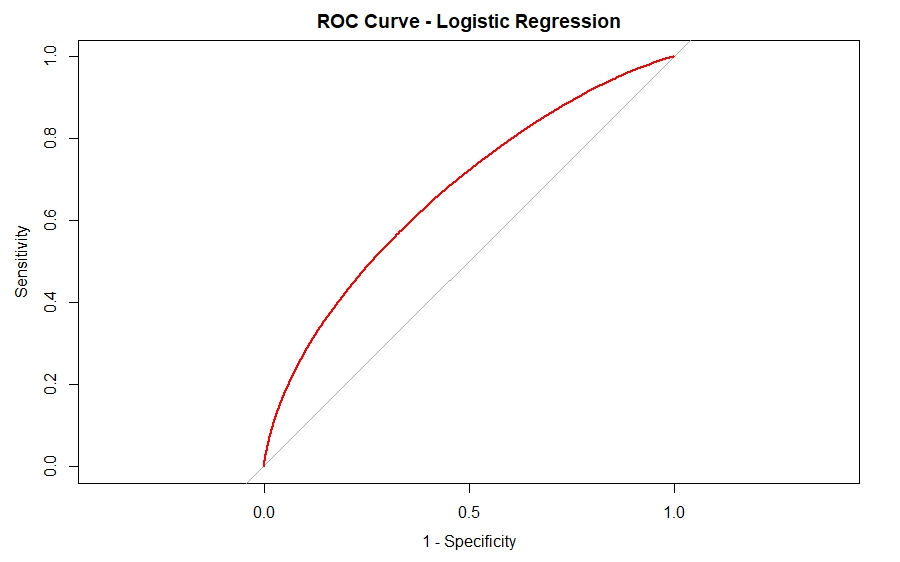
\includegraphics[width = .55 \textwidth]{../figures/PLOTS FOR REPORT/Logistic Regression/ROC Curve - Logistic Regression}
	 		\caption{Receiver Operating Characteristic Curve to determine probability cutoff threshold for logistic regression}
	 		\end{wrapfigure}
	\tab Finally, after validating our model on the testing data, we generated a confusion matrix and other measures of performance as shown in \underline{Fig X.X}. Our accuracy was 67.62\% where out of our testing set of 92,667 observations, it correctly predicted 62,187 of them. Observe from the confusion matrix that we have significantly more false positives than false negatives. Thus, we interpret this as our model is on the pessimistic side and is more likely to forecast a delay when in reality there is not one. \\

%%
	\section{Time-Based Model: Dynamic Regression}
	\tab From our exploratory data analysis, we noted that several different categorical variables related to time showed significant effects on the mean arrival time. In particular, the scheduled time of a flight had a noticeable effect on arrival delays over the course of a day. While our original linear model accounted for time-related effects by including aspects of the date and time as categorical variables, the assumptions of linear regression do not allow autocorrelation which we believed could play a role in the true model of arrival times.  For example, one could imagine that a flight that randomly arrives 10 minutes late could cause a subsequent flight to arrive $f(10)$ minutes late, where $f$ is some autocorrelation function. We also noted that the residuals did not appear to be random; i.e. not independent or identical. To adjust our model to reflect this reality, we constructed a new model: 
	\begin{center}
	$$Y_t = X_t\beta + \eta_t$$
	\end{center}
	where $\eta_t$ represents time series following an auto-regressive integrated moving average (ARIMA) model, and $X\beta$ represents a linear combination of the other (non-time-related) variables fitted against the residuals from the time series. \\
	\tab The difficulty with constructing this model was that the dataset was not originally in a time series format. We wanted our time series model to take into account daily, weekly, and quarterly seasonality. We briefly considered constructing time series on average measurements per time period, potentially split by some categorical grouping (e.g. flight routes, or carriers), but we considered the loss of information (through taking averages) too heavy of a price to pay. We wanted to construct time series data that consisted of one observation for at each time interval, with 19 time intervals per day, 7 days per week, and 91.3125 days per quarter. To do this, we used a bootstrap method, wherein we sampled with replacement from the original data, 6935 observations per year, corresponding to 6935 time periods, for 100 years, resulting in a bootstrap time series of ~700,000 observations. It is important to note that the construction of this time series precludes any long-term trends, i.e. the series is stationary from year to year. \\
			\begin{wrapfigure}{l}{0.55\textwidth}
			\centering
	 		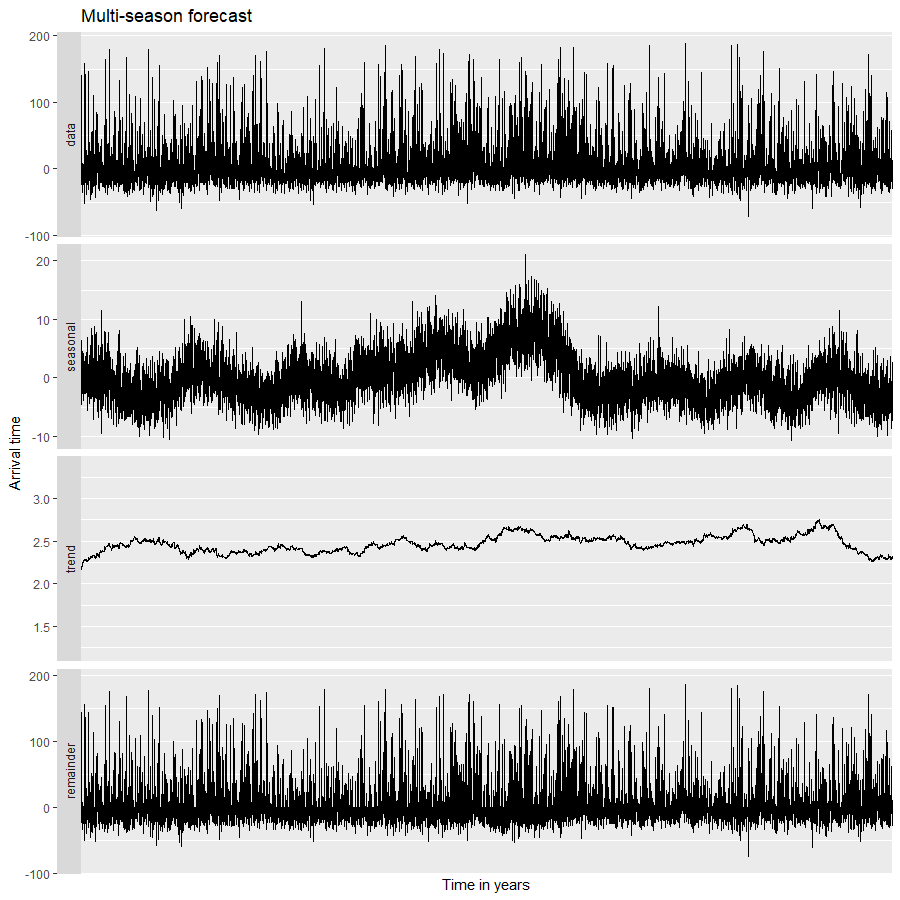
\includegraphics[width = .55 \textwidth]{../figures/timeseries_multiseason}
	 		\caption{Multiseasonal time series for arrival time, using bootstrap method}
	 		\end{wrapfigure}
	\tab Using this bootstrap time series dataset, we fitted a multiseasonal time series. Then, taking the residuals from our time series and appending it back to the original data, less arrival delays, we fitted a linear model against the residuals. The resulting model produced residuals that were approximately random, or at least more random than the previous models. A slight non-linear relationship with precipitation was observed, so the model was corrected by weighting observations by precipitation. The model parameters are described below.\\


	
%       ||||||||||||||||||||||||||||||||||||||||||||||||||||||||       CHAPTER 6 [Forecasting for 2019 Q3]
\chapter{Forecasting Flight Delays for 2019 Q3}
%%
	\section{Challenges}
	\tab Predicting flight delays is exceptionally important to facilitating economic efficiency, and for precisely that reason, it can be challenging to make predictions. As such an important topic, it is already well-trod territory, with contributions from many of the world's most preeminent statisticians. Additionally, as previously mentioned, each flight is affected by thousands of variables, each of which can potentially cause delays, either by themselves or in combination with others. Keeping track of all these variables and making predictions from them can be incredibly computationally intensive. Our exploration of the data confirms for us the inherent unpredictability of flight delays. It is clear that black swan type events are important in the genesis of flight delays, and the best types of models for accurate prediction will be able to predict those types of events. \\
	\tab However, despite our limitations, we were able to construct a dynamic linear model that explained just over 50\% of the variance in arrival delays. Our model was fit by averaging the coefficients generated by OLS on 5 separate samples of 50000 observations. 
%%
	\section{Using our Forecast Model}
	\tab To use our forecast model, we have implemented an R function that will receive an observation and generate a prediction. As previously stated, our model is of the form \begin{center}
	$$Y_t = X_t\beta + \eta_t$$
	\end{center} 
%    |||||||||||||||||||||||||||||||||||||||||||||||||||||||||          CHAPTER 7 [Business Recommendations]
\chapter{Business Recommendations}
%%
	\section{Differences Between Carriers}
	\tab As we saw in our analysis of variance in our data exploration, the average delay times across carriers do differ. More popular carriers such as American Airlines do incur more delays than say, a lesser known airline such as Pinnacle Airlines. For large carriers, Alaska Airlines and Delta do a very solid job of alleviating delays. It is also evident the more flights an airport hosts, the more chance there is at a delay occurring. From a customer’s point of view, one could simply avoid flying with the most popular airlines if the cost and quality level of another airline is adequate. From this same perspective, flying during less delay-prone times, by leaving late at night, flying during the months of January and February, or leaving on a Saturday would help families and the like minimize their chances of experiencing delays. \\
%%
	\section{Important Covariates}
	\tab As a result from playing around so much with our covariates, we gained a solid idea of what does and what doesn’t go into predicting a flight delay. Surprisingly, temperature has a minimal effect on delays, and although precipitation and weather events do contribute significantly to delays, they are rare events in the grand scheme of things, and are thus not the best way to predict future delays. On the other hand, airlines should schedule flights as to avoid propagation of delays throughout the day. Delay propagation occurs when a delayed flight early on in the day creates a ripple effect of increasingly delayed flights as the day progresses. In a sense, a delay becomes contagious as it is quite literally permeates time and spreads across the country and different airports. Thus, it is advantageous to commit resources to ensuring early flights do not get delayed. As the number of flights that take off toward the evening and into the night decreases, the airlines can catch-up during these phases to start fresh the next day. Survey data conducted on a random sample of customers could provide airlines with information regarding passengers’ willingness to fly early in the morning or late in the evening. Thus, data on clusters of passengers could be analyzed to move certain flights to different time blocks while maximizing the amount of people who would be willing to purchase tickets for these. \\
	\tab Delays simply comes down to popularity of the airport. The more balls that are thrown into the air, the more likely one will slip the hand and fall to the ground. In the end, delays will be inevitable. If airlines can predict when they will occur, then they can be more prepared to respond by compensating customers with special packages or alerting commuters further in advance about the change in logistics. 
%      ||||||||||||||||||||||||||||||||||||||||||||||||||||||||||||||        CHAPTER 8 [Closing Thoughts]
\chapter{Closing Thoughts}
%%
	\section{Retrospect}
	\tab There are many possible approaches to this type of statistical problem, so there are a plethora of algorithms and models that could end up providing the best descriptive or predictive power. Due to time and computing-power constraints, we simply employed the ones that we felt were the most efficient and promising given our circumstances. In the end, many of our critical choices were subjective. We chose our response variable, the arrival delay time, based on our own preferences and experiences with air travel. We felt that the arrival delay would be the variable of interest (as opposed to the departure delay, for example) for the majority of consumers and the most economically impactful. Choosing alternative responses such as departure delays or cancellations have their own justification. Additionally, the response could have been transformed in a number of different ways that could have made it more informative. For example, one might perhaps be interested in how long a delay will prolong only \textit{if} it occurs. Or, one could desire to know the delay time as a proportion of the original flight time. Even more, some delay metric adjusted for the distance between origin and destination could be revealing. Likewise, our choice of predictor variables was informed by our own background and objectives. For researchers with backgrounds in econometrics, it may have been more interesting to study the dataset in the context of the economic environment of 2018-2019. \\
	\tab  Technology is the other underlying component of successful statistical analysis. Being limited to our home computers for the majority of this project, we were unable to run algorithms requiring high computational loads and large memory. In such circumstances, it may have been wiser to familiarize ourselves with cloud computing services like Google Cloud's virtual machines before subjecting our own laptops to such heavy workloads. A solid amount of our models took hours and sometimes days to run. When finally finished computing, we would often need to make adjustments and re-run it again, which would require more waiting. However, overall we believe that we leveraged the available technological resources to our satisfactory.
%%
	\section{Future Work}
	\tab There are many potential analyses that can still be done on this dataset. With more computing assets, more complex machine and deep learning algorithms such as neural networks, high-dimensional clustering, and XGBoost could be applied. We believe that one of the strengths of our analysis was compiling a dataset that incorporated both the data given to us by the organizers and large amounts of outside data. In fact, we found copious amounts of downloadable outside data on airport characteristics such as runway lengths and airspace class that could have been incorporated were it not for the physical restrictions imposed by our limited RAM. \\
	\tab The question of how best to ameliorate arrival delays remains an issue of core importance to the economy. Generations of data scientists have tackled this problem, and future generations will continue to. It is obvious that the more delays are reduced, the more utility and convenience can be added to various modes of transportation (thereby raising delays again!). It is unlikely delays can be removed entirely, so the job of the data scientists is to predict them as accurately as possible. With vast and expansive amounts of data out there, the trajectories to tackle this challenge are endless. That is the beauty of big data in this new era we are in. Without a doubt, airline industries will be harnessing the power of data science, both tomorrow and forever.
%      |||||||||||||||||||||||||||||||||||||||||||||||||||||||||||||||||       CHAPTER 9 [APPENDIX]
\chapter{Appendix}
	\section{Additional Figures, Tables, Code, and Data}
%/////////////////////////////////CHAPTER 3 [Motivation, Data Desc, Software] FIGURES
			\begin{figure}[h]
			\centering
	 		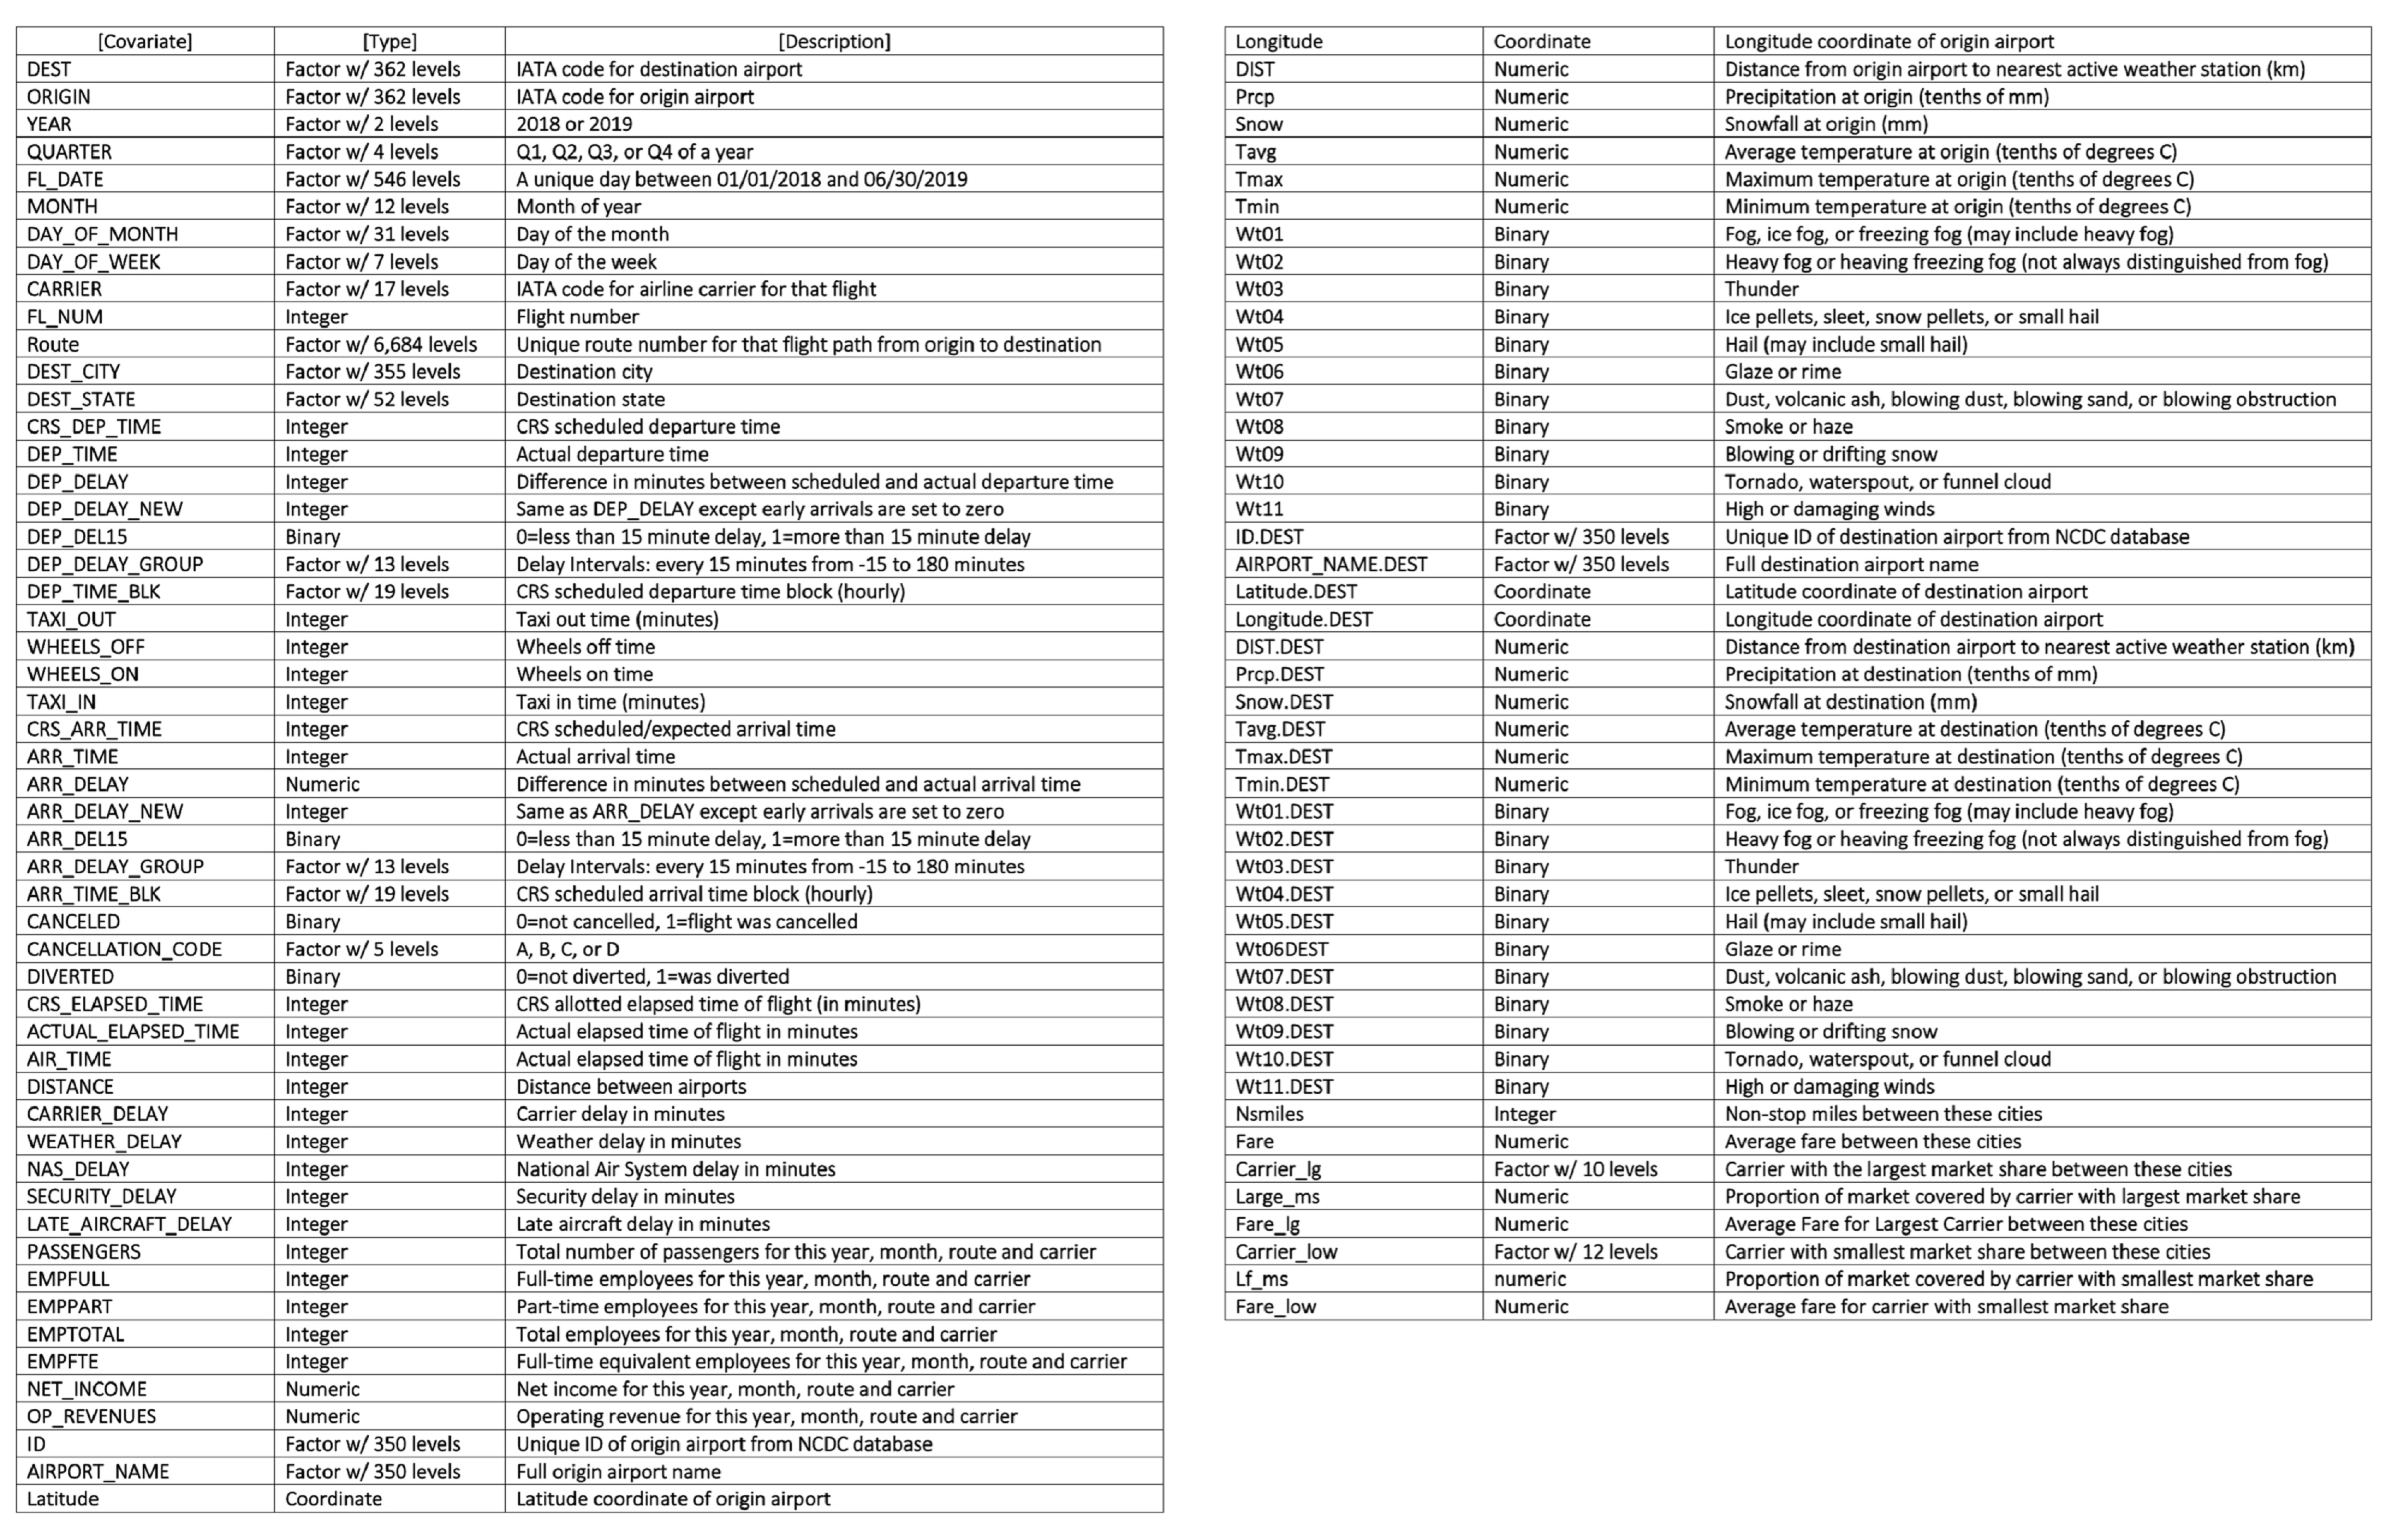
\includegraphics[width = 1 \textwidth]{../figures/PLOTS FOR REPORT/Covariate List}
	 		\caption{List of the final set of covariates along with their type and a brief description.}
	 		\end{figure}

			\begin{figure}[h]
			\centering
	 		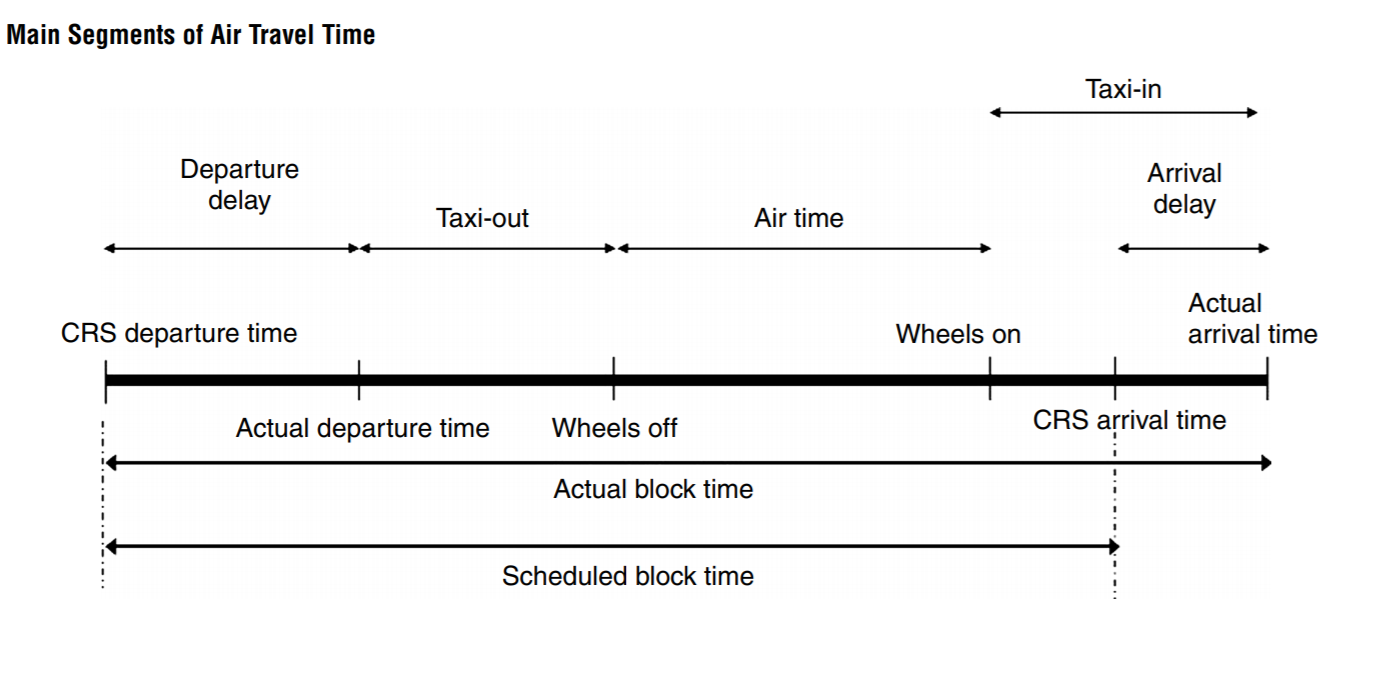
\includegraphics[width = 1 \textwidth]{../figures/Main Segments of Air Travel Time}
	 		\caption{Main Segments of Air Travel Time}
	 		\end{figure}
%/////////////////////////////////CHAPTER 4 [EDA] FIGURES
			\begin{figure}[h]
			\centering
	 		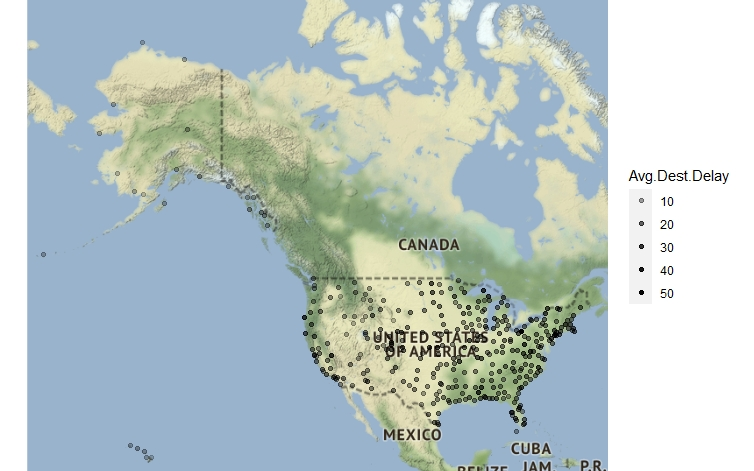
\includegraphics[width = 1 \textwidth]{../figures/PLOTS FOR REPORT/Chapter 4/Figure 4.22}
	 		\caption{Average delay at destination airports}
	 		\end{figure}

			\begin{figure}[h]
			\centering
	 		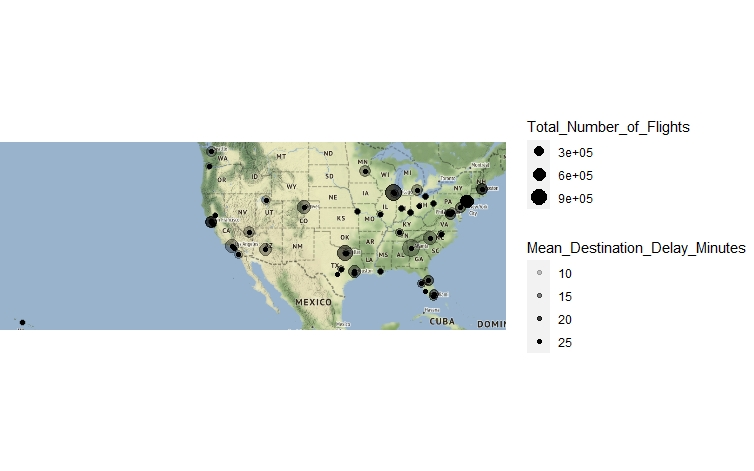
\includegraphics[width = 1\textwidth]{../figures/PLOTS FOR REPORT/Chapter 4/Figure 4.23}
	 		\caption{Average delay and total number of flights at destination airports}
	 		\end{figure}

			\begin{figure}[h]
			\centering
	 		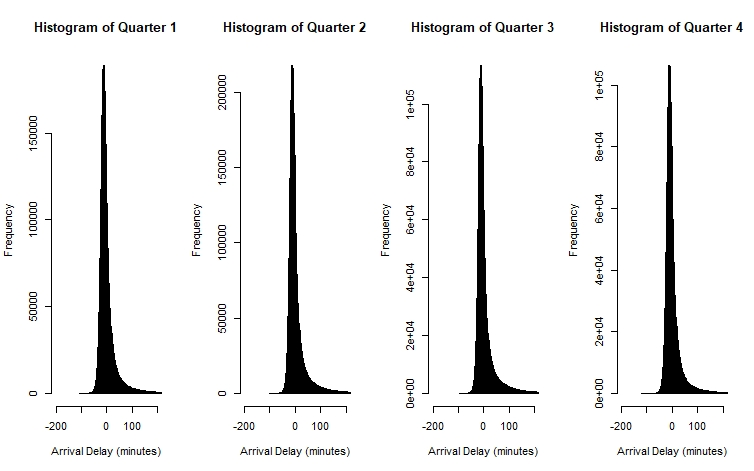
\includegraphics[width = 1 \textwidth]{../figures/PLOTS FOR REPORT/Chapter 4/Figure 4.31}
	 		\caption{Delays by quarter}
	 		\end{figure}

			\begin{figure}[h]
			\centering
	 		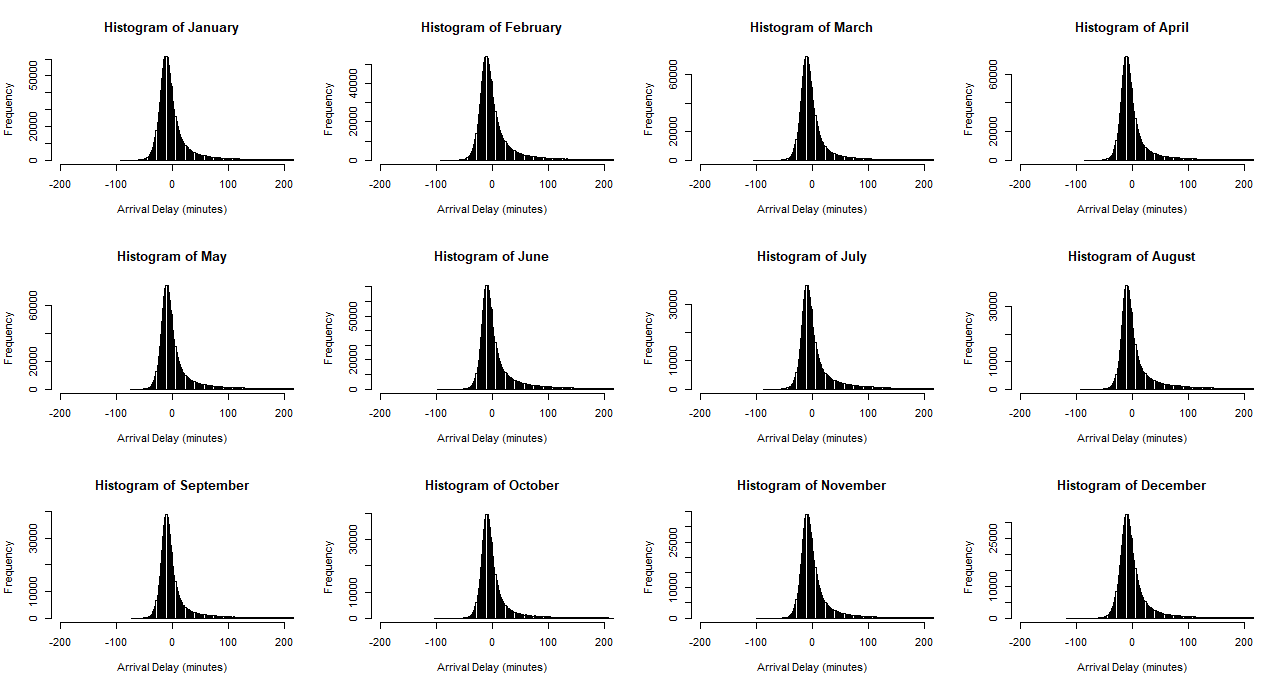
\includegraphics[width =1\textwidth]{../figures/PLOTS FOR REPORT/Chapter 4/Figure 4.32}
	 		\caption{Delays by month}
	 		\end{figure}

			\begin{figure}[h]
			\centering
	 		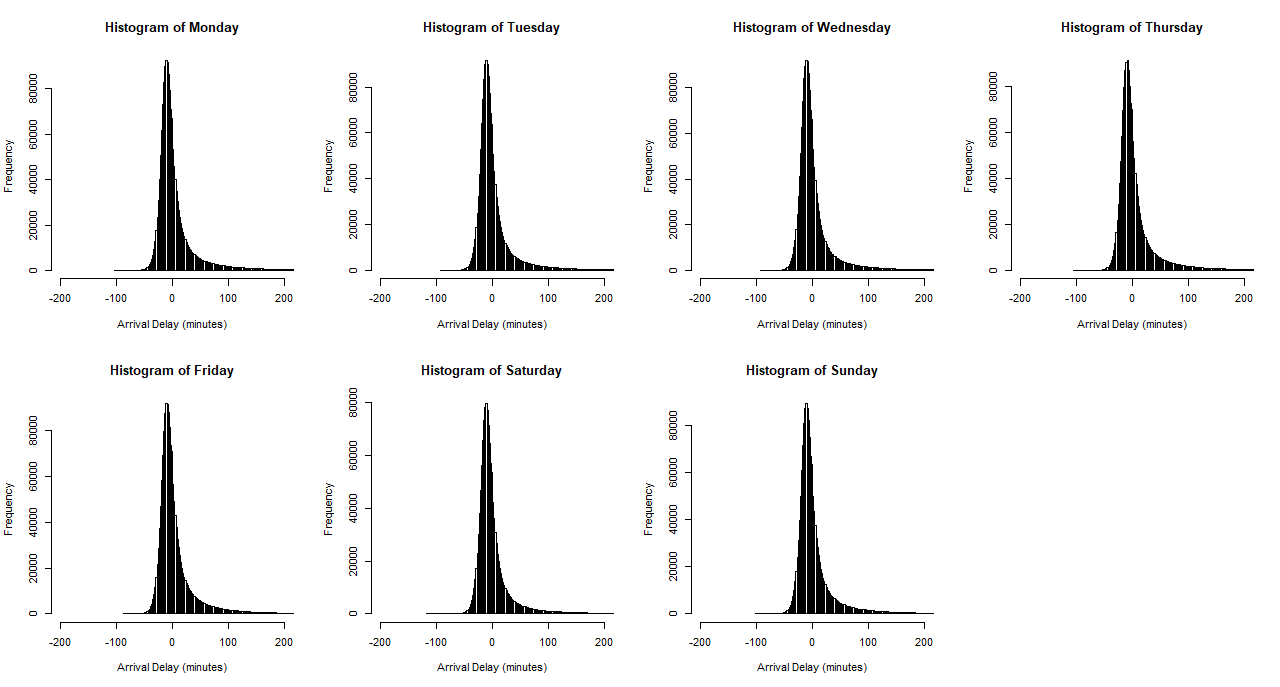
\includegraphics[width = 1 \textwidth]{../figures/PLOTS FOR REPORT/Chapter 4/Figure 4.33}
	 		\caption{Delays by day of the week}
	 		\end{figure}

			\begin{figure}[h]
			\centering
	 		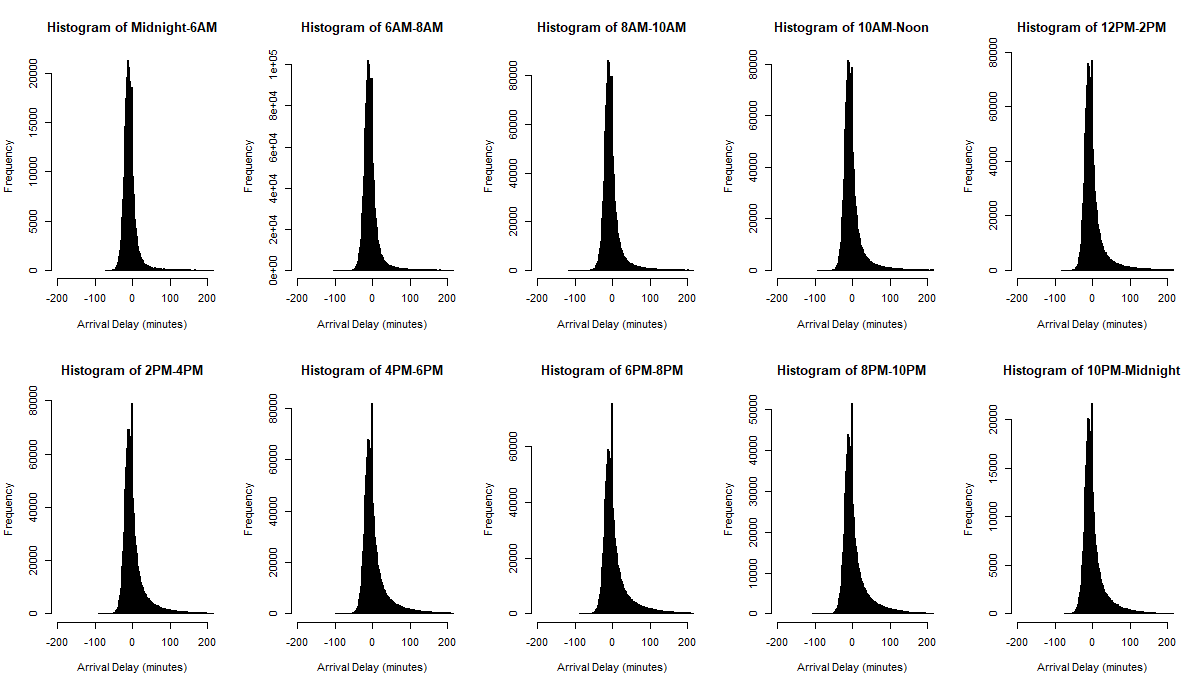
\includegraphics[width = 1\textwidth]{../figures/PLOTS FOR REPORT/Chapter 4/Figure 4.34}
	 		\caption{Delays by time of day}
	 		\end{figure}

			\begin{figure}[h]
			\centering
	 		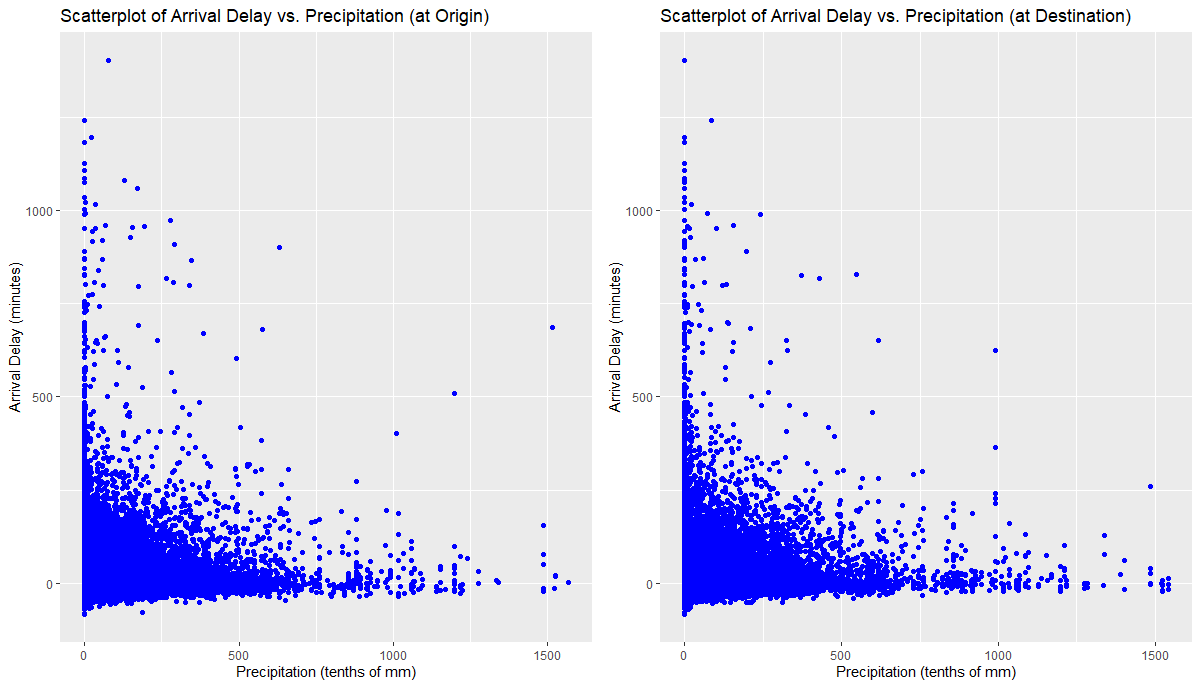
\includegraphics[width = 1 \textwidth]{../figures/PLOTS FOR REPORT/Chapter 4/Figure 4.42}
	 		\caption{Delays vs Precipitation}
	 		\end{figure}

			\begin{figure}[h]
			\centering
	 		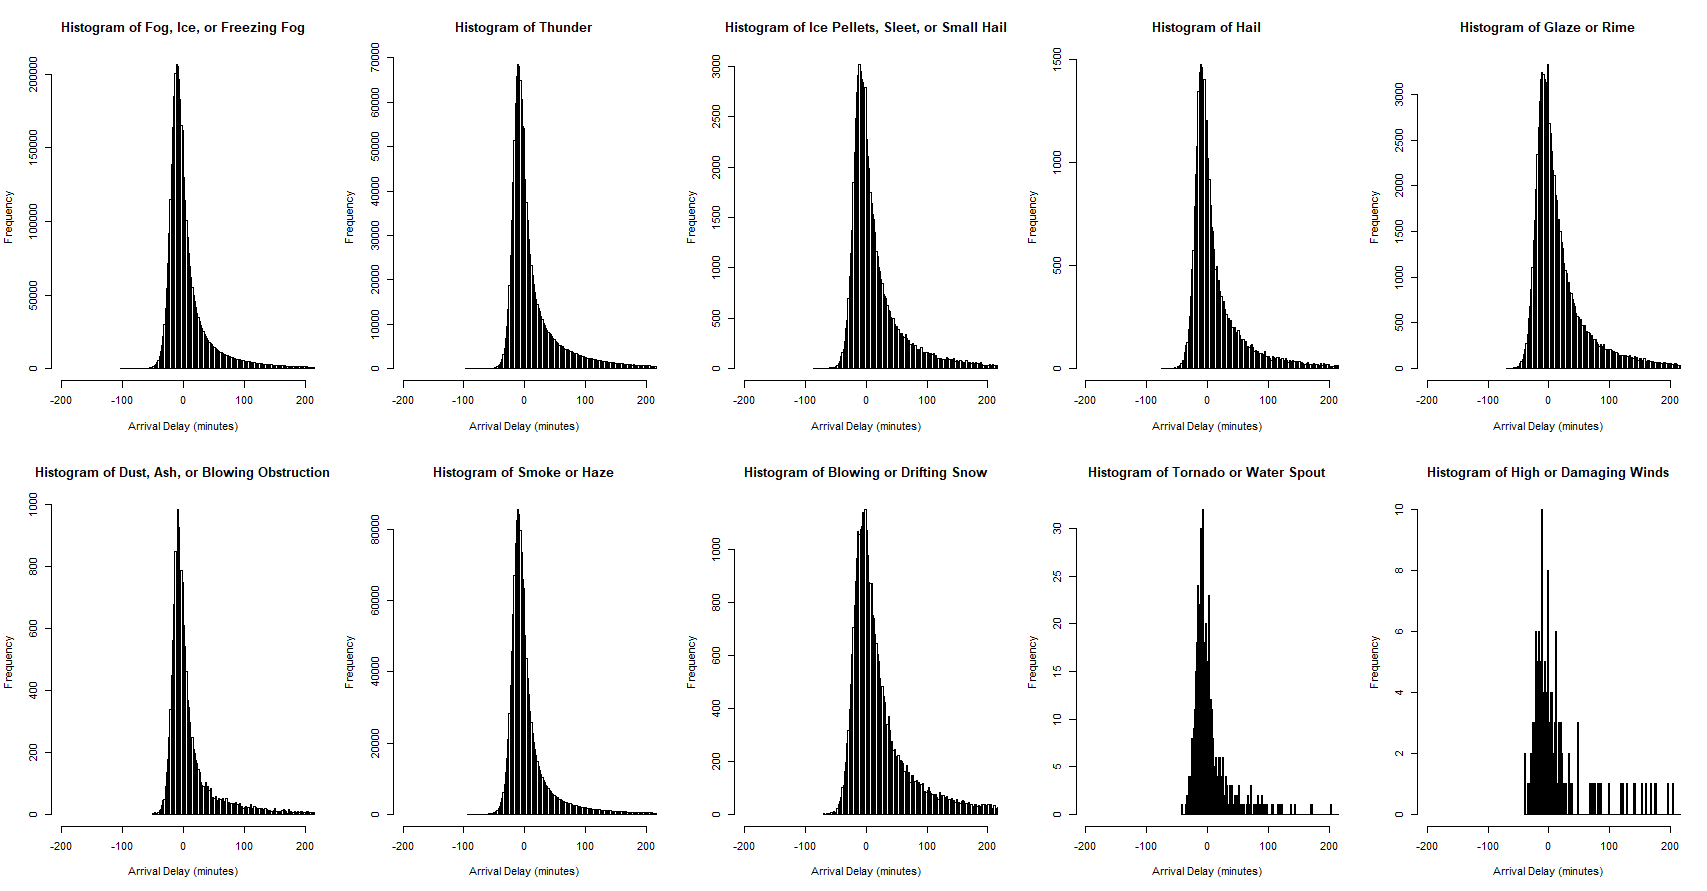
\includegraphics[width = 1 \textwidth]{../figures/PLOTS FOR REPORT/Chapter 4/Figure 4.43}
	 		\caption{Delays by unique weather event}
	 		\end{figure}

			\begin{figure}[h]
			\centering
	 		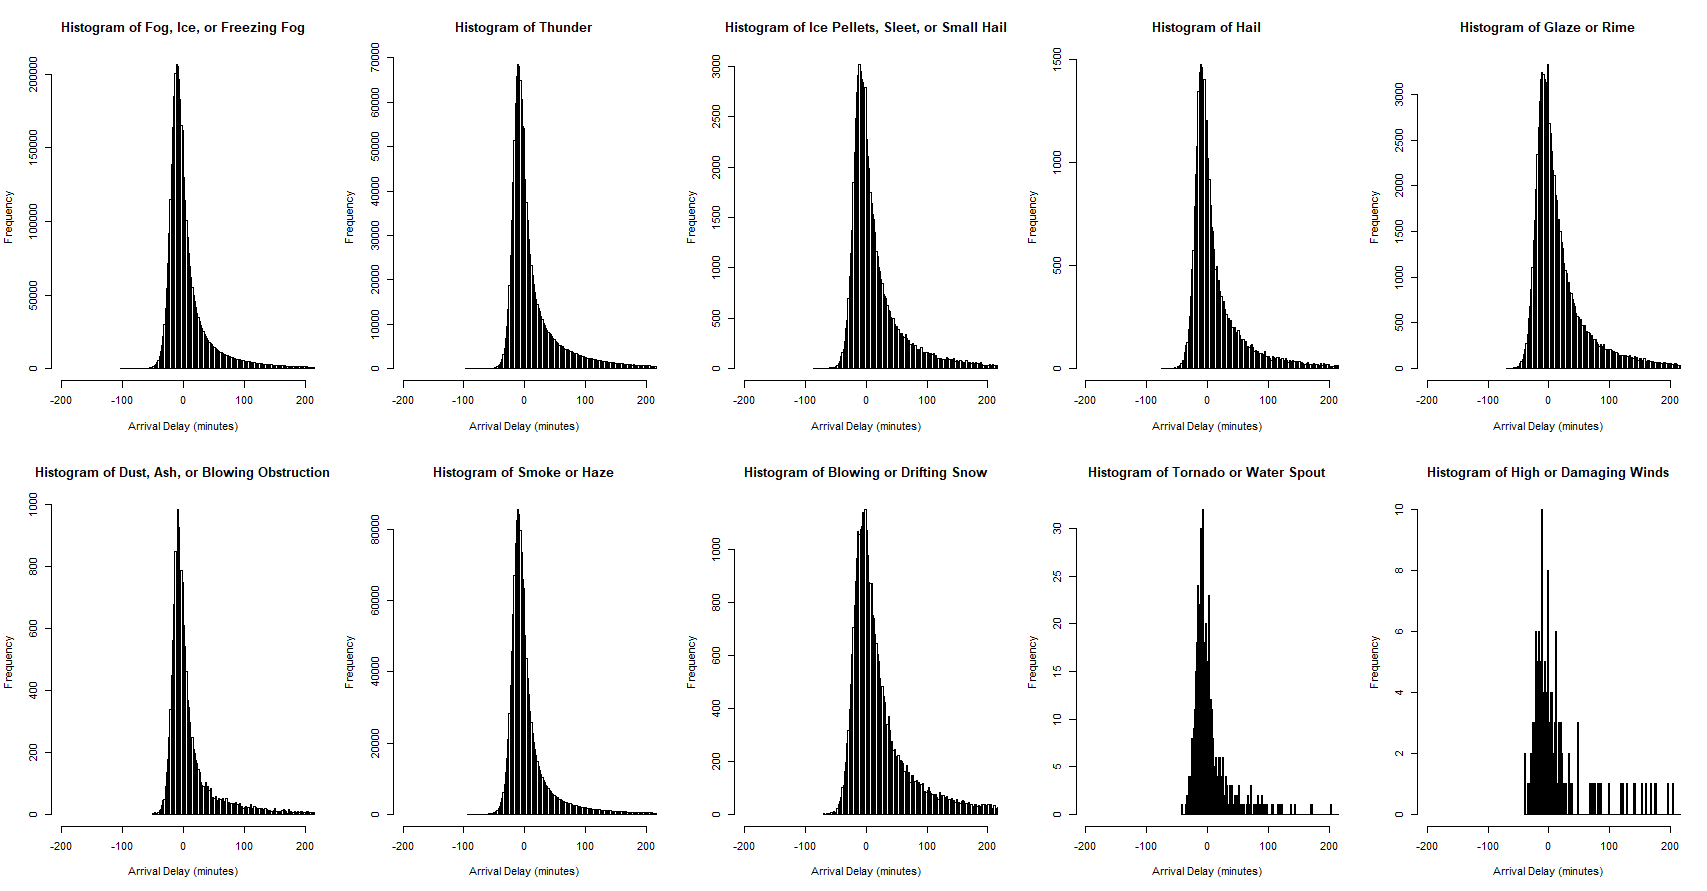
\includegraphics[width = 1\textwidth]{../figures/PLOTS FOR REPORT/Chapter 4/Figure 4.5}
	 		\caption{Delays by carrier}
	 		\end{figure}

			\begin{figure}[h]
			\centering
	 		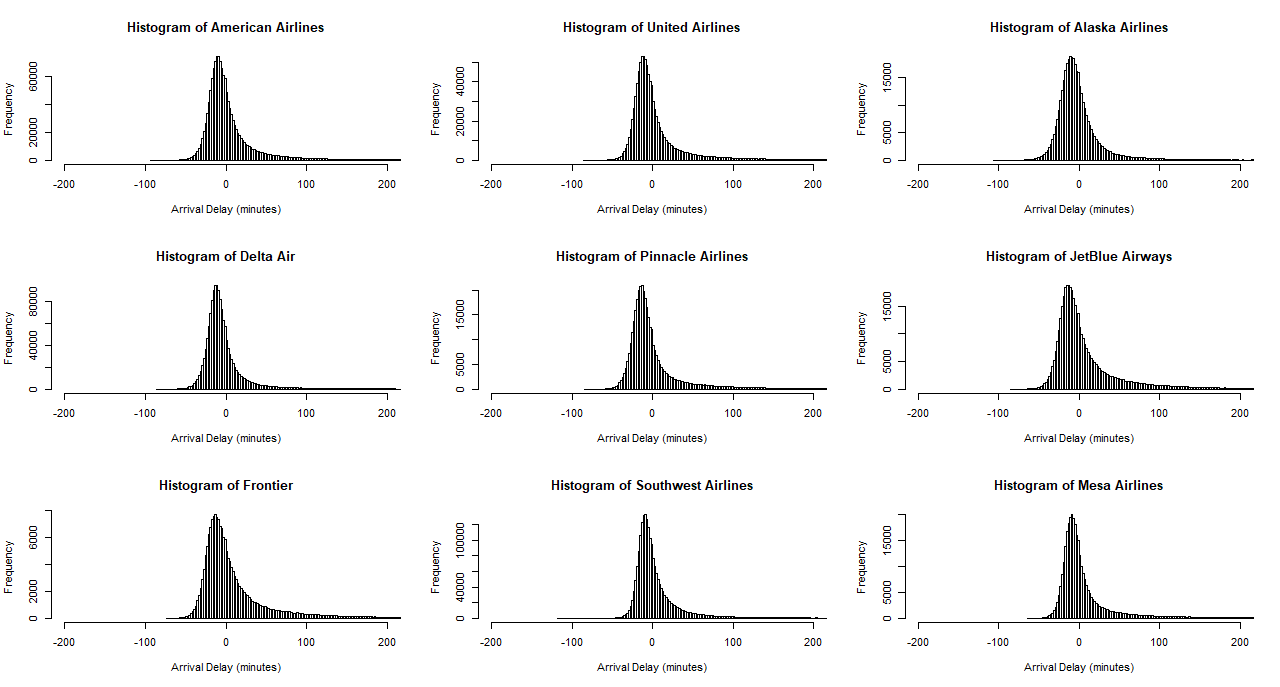
\includegraphics[width = .9 \textwidth]{../figures/PLOTS FOR REPORT/Chapter 4/Figure 4.6}
	 		\caption{Tukey's HSD: 95\% Confidence Intervals for the difference in mean delays across carriers}
	 		\end{figure}

			\begin{figure}[h]
			\centering
	 		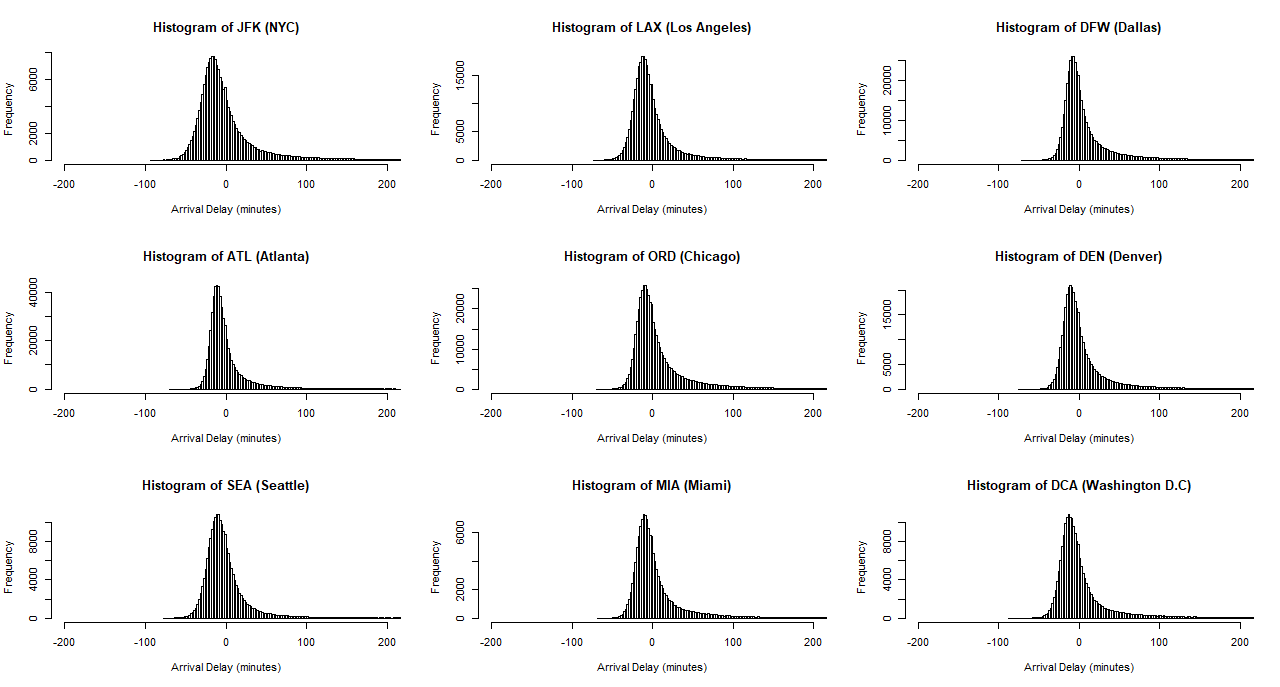
\includegraphics[width = 1 \textwidth]{../figures/PLOTS FOR REPORT/Chapter 4/Figure 4.7}
	 		\caption{Delays by airport}
	 		\end{figure}

%/////////////////////////////////CHAPTER 5 [MODEL FORMULATION AND ASSESSMENT] FIGURES

			\begin{figure}[h]
			\centering
	 		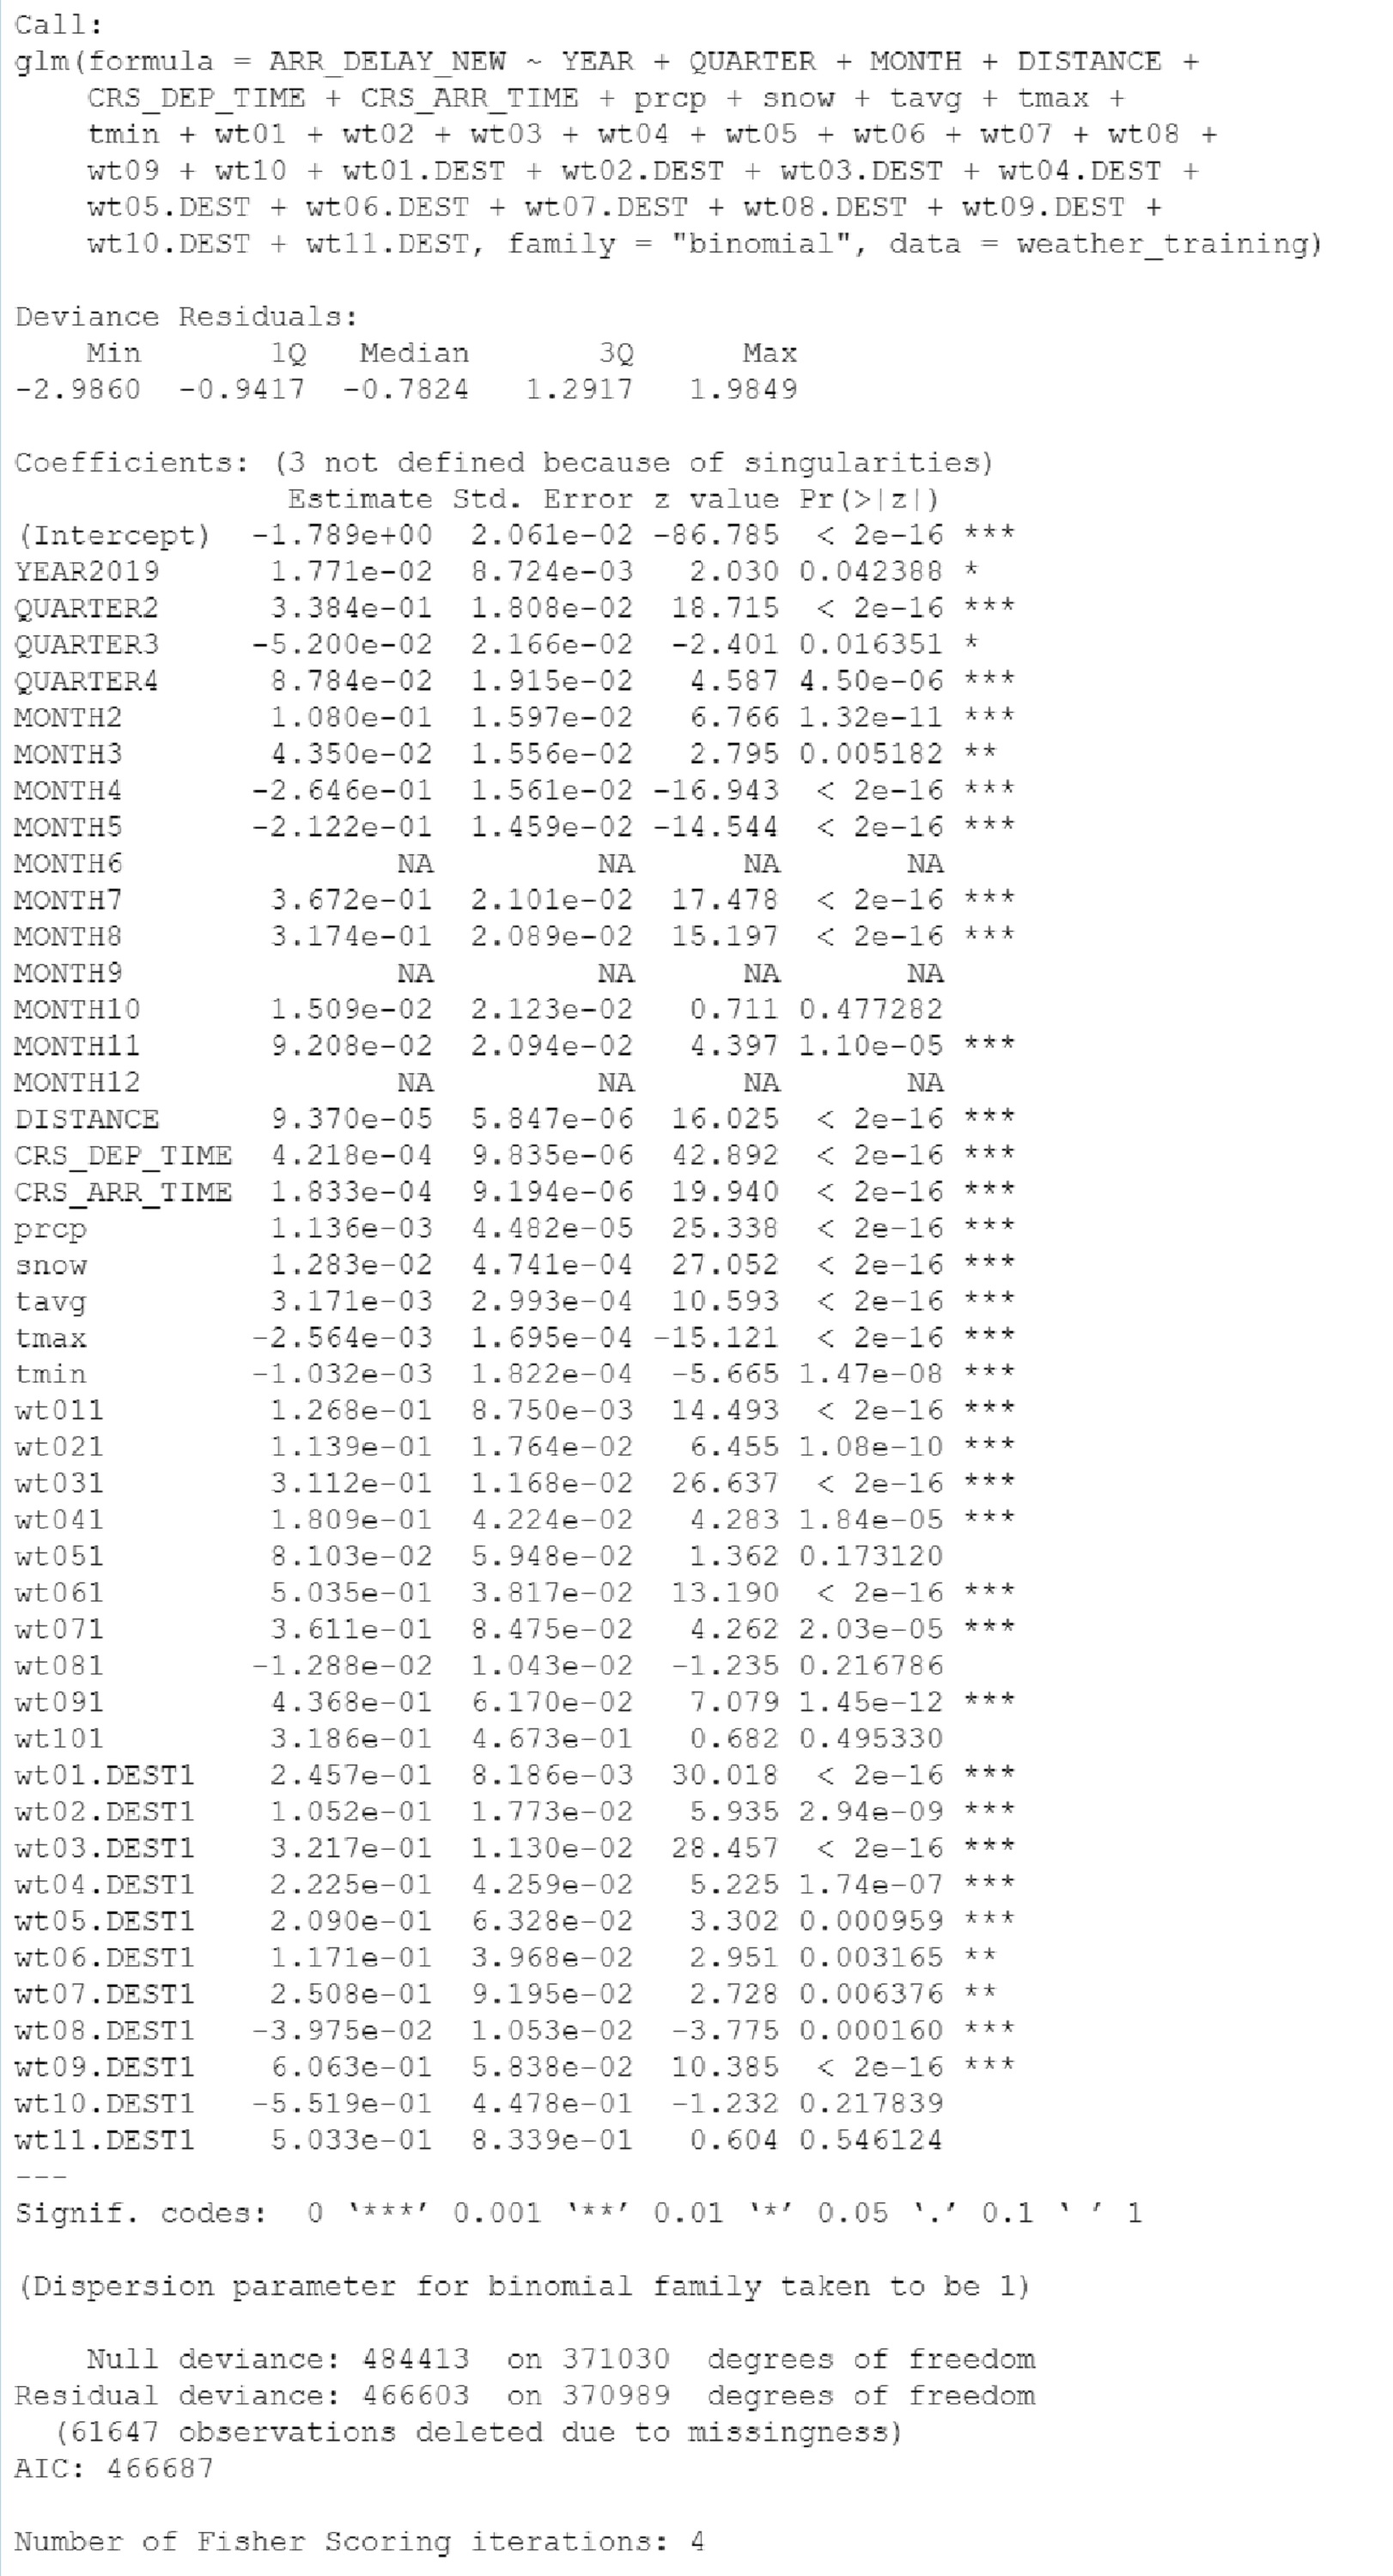
\includegraphics[width = .8\textwidth]{../figures/PLOTS FOR REPORT/Logistic Regression/summary(logit_reg)}
	 		\caption{R output for logistic regression}
	 		\end{figure}

			\begin{figure}[h]
			\centering
	 		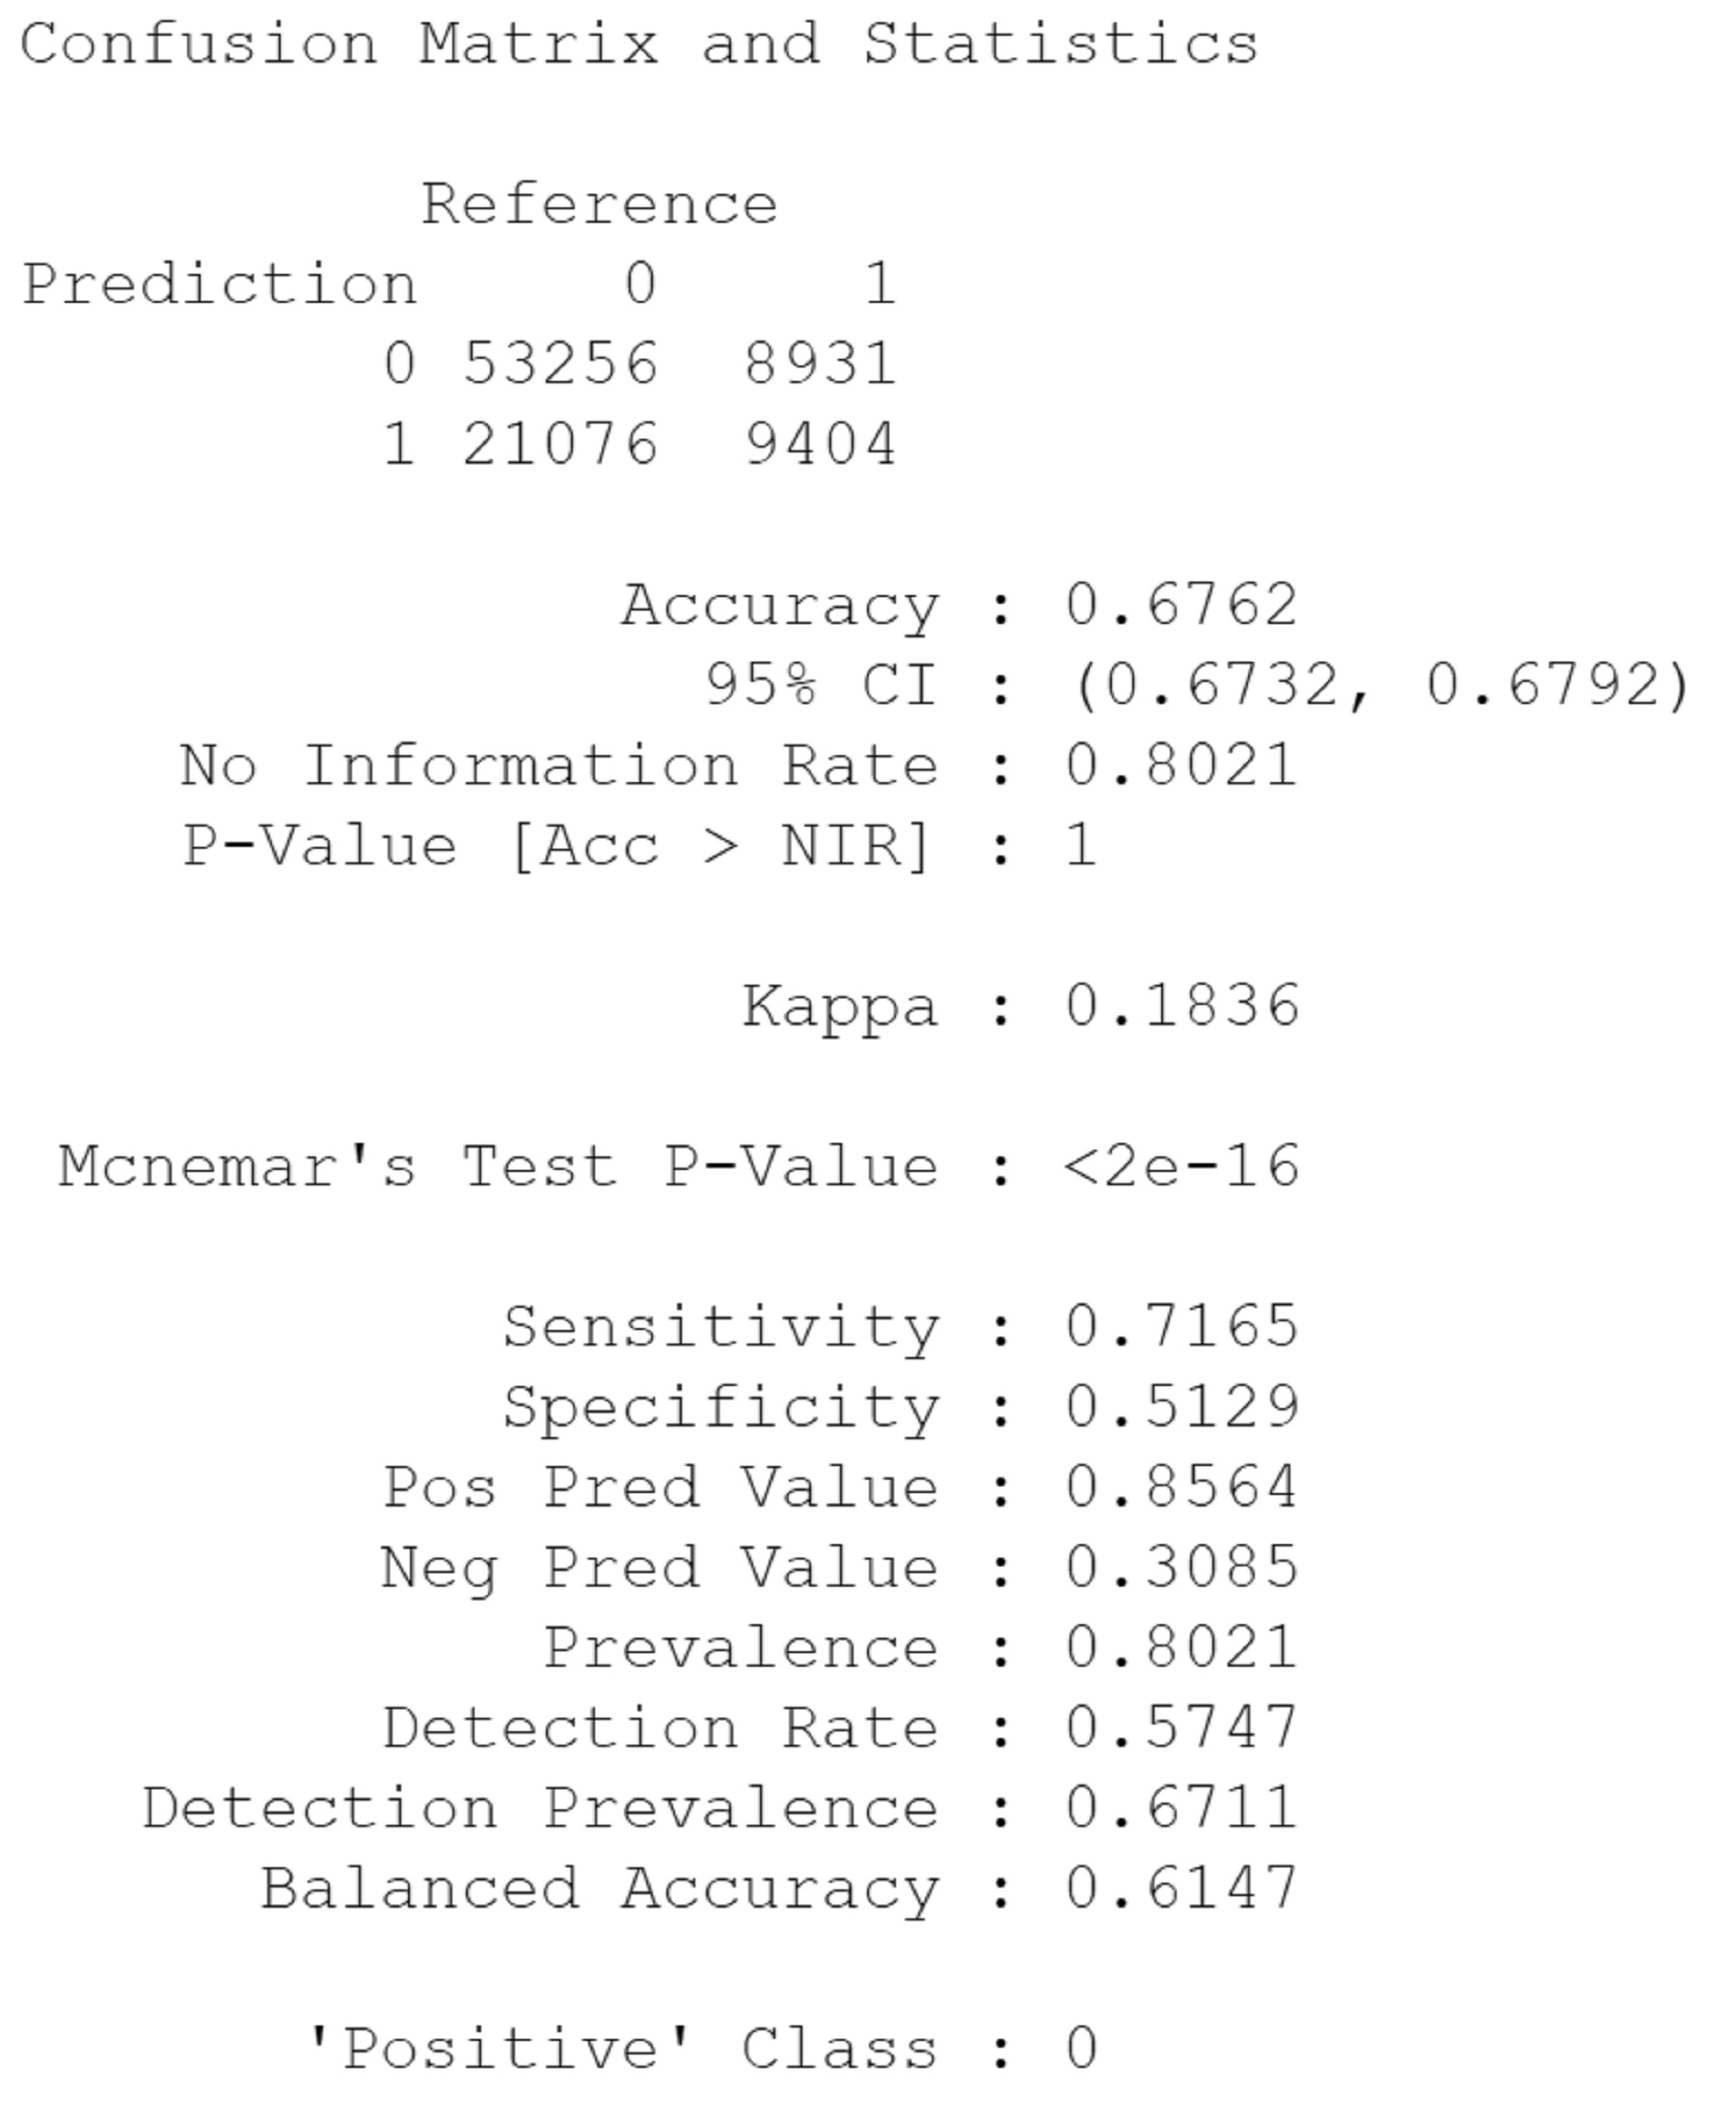
\includegraphics[width = .45\textwidth]{../figures/PLOTS FOR REPORT/Logistic Regression/confusion matrix - logit reg}
	 		\caption{Confusion matrix and other performance measures for logistic regression}
	 		\end{figure}

\pagebreak

\bibliographystyle{natdin}
\nocite{*}
\bibliography{sources}
\end{document}